\chapter{User Scheduling via Manifold Clustering} \label{chap:U-SCH}

In this chapter we propose and design a novel, simple, and practical unsupervised learning approach to MAC user scheduling based on uplink CSI knowledge.
Unlike supervised learning, which would require a large number of labeled training channels, our unsupervised MAC user scheduling can directly operate on knowledge of user uplink channel state information (CSI) to mitigate multiple access interference (MAI) among users and to achieve high MAC capacity. 
Our novel methodology starts by classifying users into high similarity groups through learning based on a novel metric of projected CSI similarity. 
We then develop a simple MAC protocol by only scheduling users from user groups with high inter-cluster distance for joint access to mitigate multiple access interference (MAI). 
We provide comprehensive performance evaluations of the proposed  MAC scheduling protocol in terms of spectral  efficiency, bit-error-ratio, user fairness, and robustness.


In the Internet-of-Things (IoT) era, tens of billions of wireless devices will be connected around the globe \cite{Qualcomm15, Andrews14}. 
The tremendous growth rate of wireless communication networks in areas such as transportation, environmental monitoring, robotics, and smart cities continue to demand higher 
spectrum efficiency over the limited
bandwidth resources.
Multiple-Input-Multiple-Output (MIMO) technologies have been playing a central role in achieving high
network throughput and spectrum efficiency \cite{LTE12}
in both uplink and downlink transmissions.
In uplink multiple access channel (MAC), classical multi-user detection (MUD) receivers such as the maximum-likelihood, zero forcing, minimum mean square error, or decision-feedback detectors (and derived techniques) allow to recover simultaneous recovery of multiple signals over the same physical resource
\cite{Verdu1986a,Vandenameele00, Hanzo03,Verdu1986b, Xu02,Verdu89, Xie90, Madhow94,Heath05}. Similarly, MU-MIMO
enables shared spectrum and high efficiency in downlink \cite{mu-mimo2012}.

Despite the high popularity and broad application of uplink MAC and downlink MU-MIMO systems, 
their
efficiency and performance depend critically on
user scheduling algorithms.  In particular,
high spectrum efficiency requires low
mutual interference among co-channnel
users scheduled for MU-MIMO downlink or 
MAC uplink. 
The ultimate goal of \emph{scheduling} is to know how to assign users such that they share the most resources without sacrificing performance (measured in any metric of interest: sum-rate, capacity, outage probability, among others), i.e. with minimal interference \cite{Goldsmith2003}. In other words, scheduling aims to identify
co-channel users with minimal or controlled co-channel interference (CCI). 

In MIMO systems, CCI depends directly on spatial channel diversity among sources \cite{Eduardo17, Maciel10}, i.e., on 
user channel similarities. 
The spatial diversity needs to be assessed 
based on regular channel state information 
(CSI) update. 
For a base station with $M$ antennas and
single antenna mobile devices, 
up to $M$ users can be scheduled simultaneously
in MIMO downlink or uplink co-channel
users. The co-channel user CSI vectors 
must exhibit sufficient linear independency \cite{Hong03, Shiu00}. 
However, to optimally schedule users in resource-sharing groups, one needs to examine the CSI matrix of each possible group over the user set. 
Given the large number
of serviced devices $N$ and increasing large
number of base-station antennas $M$, the 
number of user scheduling options is of order
$\mathcal{O}(N^M)$. 

Since MIMO user scheduling is a combinatorial, NP-hard problem, even for a moderate number of users (e.g. dozens or hundreds),  
existing algorithms are typically heuristic.
For example, some recent methods take advantage of proportional fairness (PF) and the determinant pairing algorithm (DPS) \cite{Chen08, Chang16, wang11}. However, these schemes rely in exhaustive computation of spatial cross-correlations for various possible user groups, and as such require heavy computational workload. 

Other approaches exploit localized characteristics, in the sense of  characteristics shared among small subsets of users that can be easily computed. One trend examines the pairwise CSI correlations of all users and proposes to divide users into groups based on a given correlation threshold \cite{Zhang05, Kim15}. 
Other schemes such as \cite{Dhanushka19, Sharath19} directly group users of similar covariance matrices, which requires more complex MUD at the BS side or pilot assignments at the user side. 
Nevertheless, information of subsets of users fail to provide a comprehensive, global notion of the desired characteristics on the set of all users: in the case of pairwise correlation, it is possible to have several users that enjoy low pairwise correlation and still suffer from significant interference as they might be linearly dependant, which is even accentuated when considering several users. These localized approaches are also very sensitive to the selection order of users, as different choices might lead to wildly different performance according to the realization of CSI values. 

Recently, the use of machine learning has successfully been applied to a diverse 
array of difficult networking problems, including MAC user scheduling \cite{Kaufman90, Cui18, Morocho19, Xu14}. In fact, both supervised and unsupervised learning 
algorithms have found applications in wireless CSI characterization \cite{Jiang17} that 
can facilitate user scheduling. 
In the context of wireless communications, supervised learning 
demands a rich training database consisting of diverse CSIs and 
corresponding labels of scheduled user groups. The reality is
that there are no known ``optimum scheduling''
labels in existence to account for 
large varieties of CSI characteristics, 
and different system settings such as
number of antennas, number of users, 
type of wireless channels, various noise
levels, different user power constraints.
For this reason, building a large labeled training
set itself for supervised learning is highly challenging,
particular for a rich variety of dynamic scenarios involving
a large number of users. 

In contrast, unsupervised learning does not require labeled training data and 
aims to explore underlying shared characteristics among data points
without having to know beforehand which are vital features to extract. 
Importantly, unsupervised learning can effectively identify user CSIs that are highly similar. 
However, MAC and BC user scheduling requires to identify users with highly dissimilar CSIs as co-channel groups to mitigate 
mutual interference. Therefore, unsupervised learning 
is not directly suitable for user scheduling, as most existing 
proposals incorporate additional rules and criteria to compensate
this shortcoming. 
% Such strategies require the formation of CSI clusters based on CSI dis-similarity rather than more naturally on CSI similarity. Hence, a laissez faire adoption of traditional learning algorithms for MAC user scheduling is generally ineffective because of the clear incompatibility between what learning is designed to do, i.e., to learn shared features, and what MAC user scheduling requires, i.e., forming MAC user groups with stronger CSI dis-similarity. 
For example, the authors in \cite{Cui18} propose a user clustering algorithm based on CSI correlation, in which a new user arrival would select a user cluster among existing clusters corresponding to minimum Euclidean distance to its beamforming vector to reduce inter-beam interference.
In \cite{Xu14} the authors focus on user grouping in massive MIMO in accordance to various clustering methods. 

Hence, any desirable and general user scheduling approach should tackle the following question:
How to globally determine satisfactory user groups for efficient scheduling, with reasonable complexity? Equivalently, the problem 
is to identify group users with 
sufficiently distinct CSIs 
scheduling MAC or BC users.
Here, there are two key aspects to address. First, such a scheduling approach requires to analyze the whole dataset rather than part of the dataset. More importantly, this would require a quantitative notion or measure of dissimilarity to be applied globally, and this is not qualitatively pre-defined: 
any such measure should be 
dynamically adaptive and scalable 
to account for various forms and degrees of dissimilarity, which is both hard and could be computationally intensive.

Although
user CSI dissimilarity is difficult to
quantify, we note that CSI similarity is well defined. For example, high crosscorrelation
between two CSI vectors would directly 
lead to strong mutual interference in MAC or BC.
Thus, we present a different approach to user
scheduling in this work.  Instead of trying
to identify dissimilar user CSIs in
co-channel user scheduling, we
would develop a scalable and dynamic algorithm
to \emph{first} identify users with highly \emph{similar} CSI.
By prohibiting users with highly similar CSI as co-channel MAC or BC users, we can then schedule users that do not fall within the same CSI similarity set. 

In this paper, we present a principled two-step strategy based in this problem reformulation, where we leverage the power of unsupervised learning and incorporate domain knowledge by defining how user CSIs are similar in the sense of linear independence when grouping users, redefining the geometry of the CSI space to a Riemannian manifold such that similarity is an inherent measure of the dataset, and later exploiting the similarity information to improve scheduling as it provides guidelines on how it is more convenient to group or not group a particular subset of users. 

We organize this manuscript as follows. Section~\ref{sec:USCH_systemmodel} presents the signal model for user scheduling, CCI and system performance metrics.
Section~\ref{sec:USCH_strategy} introduces our general strategy for unsupervised user scheduling, 


\section{System model and Problem Statement}\label{sec:USCH_systemmodel}
\begin{figure}[tb]
	\centering
	% requires \usepackage{graphicx}
	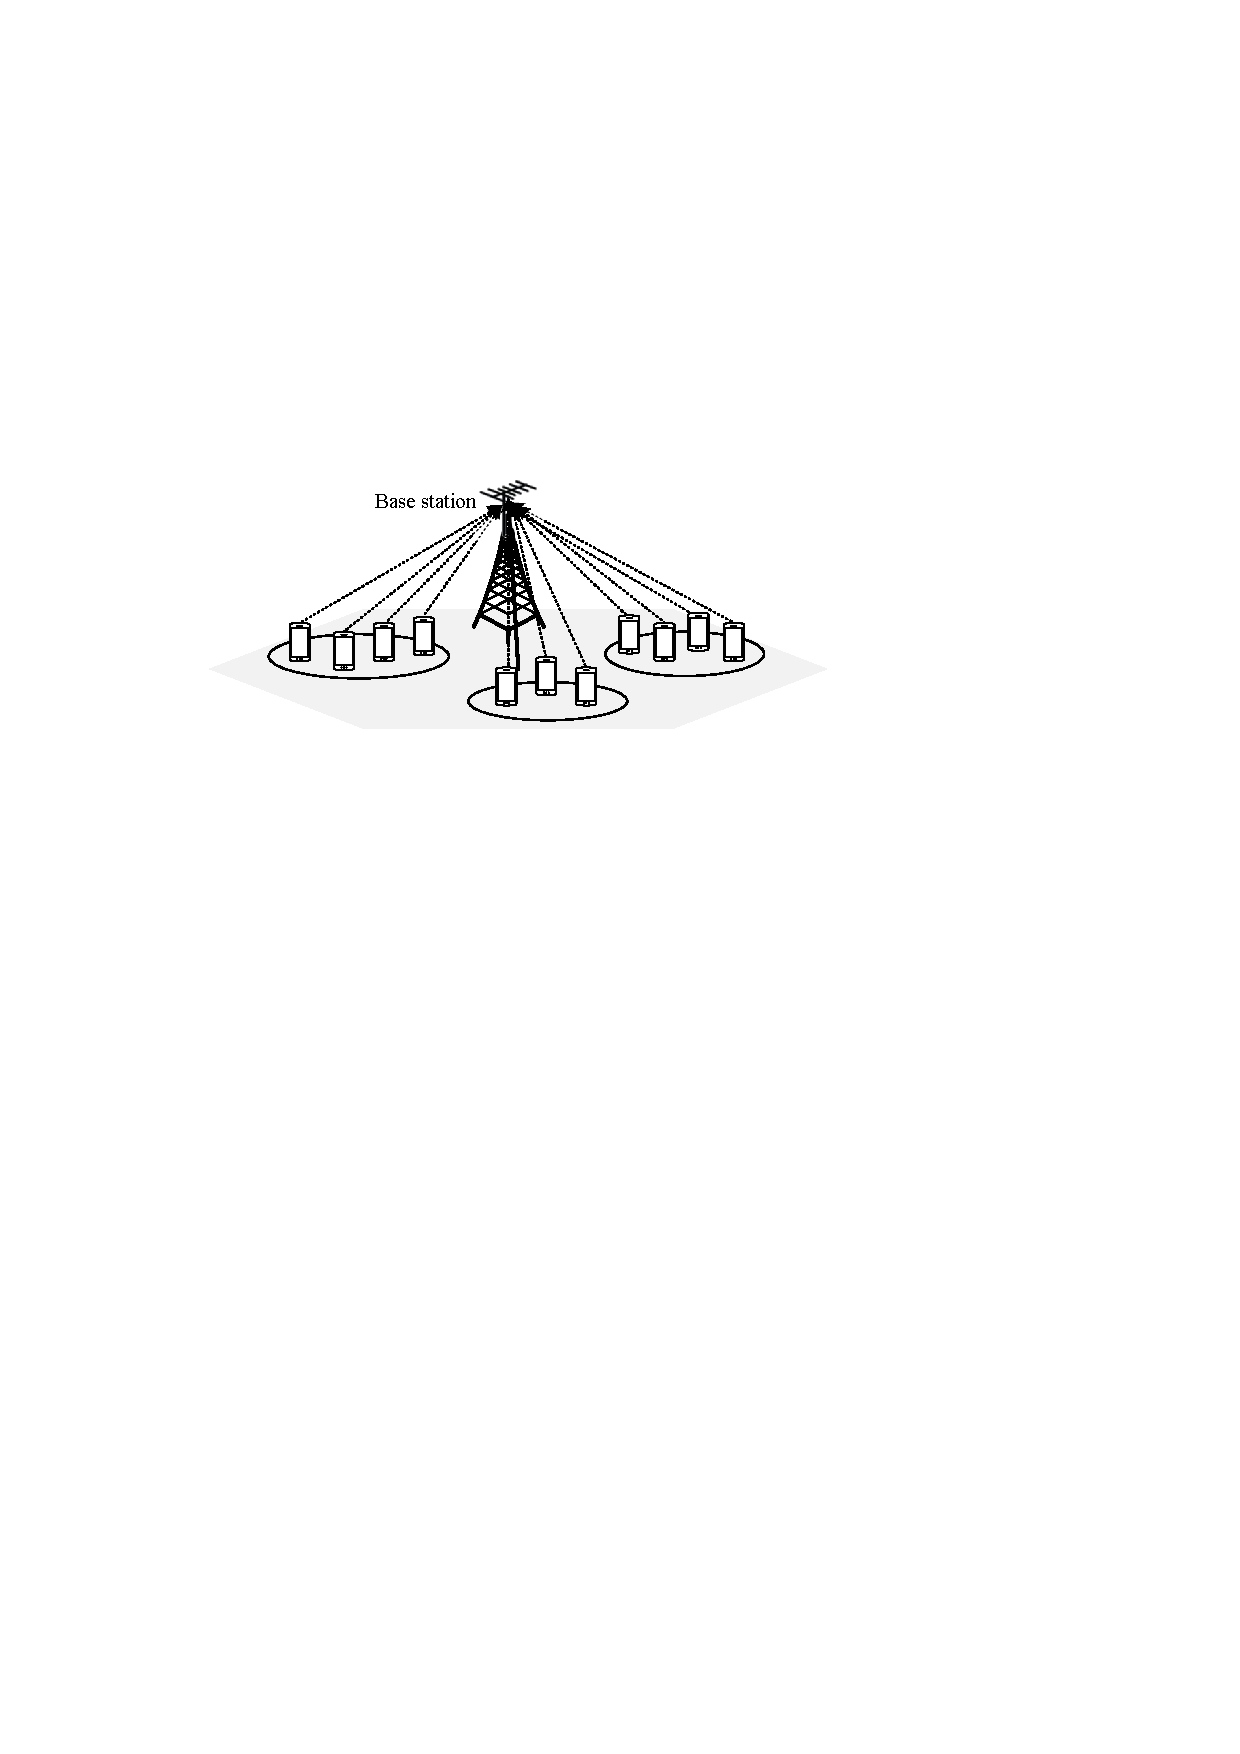
\includegraphics[width=0.45\textwidth]{usch_figs/system_model_0911.pdf}\\
	\caption{\textcolor{black}{Illustration of user scheduling for spatial multiplexing. Users in the same group deliver (MAC) or receive (BC) independent signals in a multiplexing mode on the same time-frequency resource.}}\label{fig:usch_system_model}
\end{figure}

Fig.\ref{fig:usch_system_model} depicts a wireless system with a single BS with $M$ receiver antennas and $N$ single-antenna users. We assume $N\ge M$ and a single-carrier system. Without loss of generality, we consider Time Division Multiple Access (TDMA) where different spectrum-sharing groups can be allocated into distinct time slots. Other access mechanisms, such as FDMA or OFDMA, can also be considered with proper CSI models.

In the case of MAC, the BS has access to the CSI of active users, and therefore it shall determine user scheduling. 
Furthermore, to ensure linear independence of grouped users, the joint detection of multiple MAC user signals by the multi-antenna BS requires that resource-sharing groups have at most $M$ users. 
% The MAC user scheduling task can be stated as follows: 
% Given $N$ active MAC users and their uplink CSIs, assign all users into multiple uplink MAC user groups of size up to $M$ in a BS-coordinated network.

For a BC system, we assume that the BS has knowledge of the users' CSI either by the use of a separate feedback channel, or under time-division duplexing (TDD) due to channel reciprocity. All other considerations remain the same, and the BS also manages user scheduling. 


\subsection{A General System Model} 

Let $\bm{h}_{n}\in \mathbb{C}^{M}$ be the uplink/downlink CSI vector of the $n$-th user. We assume the CSIs are random and independent from each other.
%$\bm{h}_{m} = \bm{z}_m d_m^{ -\alpha/2}$. Here, $\bm{z}_{m}\in\mathbb{C}^{N}$ corresponds to small Rayleigh fading coefficient of user $k$, i.e., $\bm{z}_{m}\sim\mathcal{CN}(\bm{0},\bm{I}_{N})$. The last factor captures the long-term/large-scale fading, i.e., path-loss and log-normal shadowing, $d_{m}$ is the distance between user $m$ and the BS, and $\alpha$ is the path-loss exponent. 
Let $G$ the total number of groups to be assigned, and let $\pi_{g,n}\in\{0,1\}$ indicate whether the $n$-th user is scheduled in group $g\in\{1,\ldots,G\}$ exclusively, i.e.
\begin{equation}
	{\pi _{g,n}} = \left\{ \begin{array}{ll}
		1&\text{the $n$-th user belongs to group $g$ only,}\\
		0&\text{otherwise,}
	\end{array} \right.
\end{equation}
and  $\bm{\Pi}_g=\diag(\pi_{g,1},\ldots,\pi_{g,N})\in\{0,1\}^{N\times N}$ the matrix that collects all indicators of group $g$ in its diagonal.

Furthermore, the set $\mathcal{S}_g=\{n|\pi_{g,n}=1, n\in\{1,\ldots,N\}\}$ 
denotes the scheduled
user set of the $g$-th group with cardinality
$|\mathcal{S}_g|$.
Finally, we define $\bm{\Pi}=\{\bm{\Pi}_g\}_{g=1}^G$ as the set of indicator matrices.

% For convenience, we also define $\bm{\Pi}_g\in\mathbb{R}^{N\times |\mathcal{S}_g|}$ which denotes the user scheduling matrix of group $g$ as
% \begin{equation}
%     \bm{\Pi}_g=\begin{bmatrix}\bm{e}_n\end{bmatrix}_{n\in\mathcal{S}_g},
% \end{equation}
% and note that 
% \begin{equation}
%     \bm{\pi}_g\bm{\pi}_g\herm=\bm{\Pi}_g\bm{\Pi}_g\herm=\diag\left(\bm{\pi}_g\right)\in\mathbb{R}^{N\times N}.
% \end{equation}

\subsection{MAC (Uplink) Scenario} 

In MAC uplink, let $x_{n}$ denote the $n-$th user data symbol of zero mean and unit average power, i.e. $\mathbb{E}\left[ {|{x_{n}}|^2} \right] = 1$. 
Let $p_n$ represent the transmit power of the $n-$th user.
At the BS, the $|\mathcal{S}_g|$ user signals from the scheduled MAC user group $g$ arrive at the BS receiver through their respective channel responses $\{\bm{h}_n\}_{n\in\mathcal{S}_g}$ to generate the received signal vector
\begin{align}\label{eqn:sig_mac}
	\bm{y}_g^{\MAC}&= \sum\nolimits_{n \in \mathcal{S}_g} \bm{h}_n\sqrt {p_{n}}x_{n}  + \bm{w}_g\nonumber\\
	&=\sum\nolimits_{n} \bm{h}_n\sqrt {p_{n}}x_{n}\pi_{g,n}  + \bm{w}_g\nonumber\\
	&=\bm{H}\bm{\Pi}_g\bm{P}^{1/2}\bm{x} + \bm{w}_g,
	% 	&= \bm{H}\bm{P}^{1/2}\bm{\Pi}_{g}\bm{x}  + \bm{w}_g
\end{align}
in which $\bm{w}_g\sim \mathcal{CN}(\bm{0}_M,\sigma^2 \bm{I}_{M})$ represents the AWGN vector correspoding to the resource block assigned to group $g$, and $\bm{P}=\diag(p_1,\ldots,p_N)$.
%\textcolor{magenta}{Here we can see that the dimension of $\bm{y}_g$, $N_0=\text{rank}(\bm{H}_g)\leq \min(M,N)$ is the number of parallel streams of data that is to be transmitted \cite{Sampath01}.}
%\cjferes{This is not true. The size of $\bm{y}$ will be dictated by the number of BS antennas, and it does not say a thing about the rank of the channel matrix. We can say $N_0=\mathrm{rank}$ if we want, but it does not relate necessarily to the received vector size.}
%  with zero mean and covariance matrix of $\sigma^2 {\bm{I}}_{N}$.\
% this commented part is redundant.
% \begin{subequations}
% \begin{align}
% \bm{H}_g&=\left[ {{{\bm{h}}_{m}}|\pi_{g,m}=1,\forall m} \right]_{{N {\times } {|\mathcal{S}_g|}}},\\
% \bm{P}_g &=\text{diag}\left(\sqrt{p_m}|\pi_{g,m}=1,\forall m\right),\\
% \bm{x}_g&=\left[{x_m|\pi_{g,m}=1,\forall m}\right]_{{|\mathcal{S}_g|}\times 1},
% \end{align}
% \end{subequations}
% and we can rewrite the MAC signal model (\ref{eqn:sig_mac}) as
% \begin{align}
% 	\bm{y}_g^{\MAC} = \bm{H}_g\bm{P}^{1/2}\bm{x} + \bm{w}_g.
% 	\label{eqn:sig_mac_2}
% \end{align}
% \textcolor{blue}{Note that the model in (\ref{sig}) is indeed very general and widely used in MIMO systems.}

\subsection{BC (Downlink) Scenario} 

In the case of BC, we operate under equal assumptions. However, the signal model changes as the single-antenna receivers will experience CCI but will not be aware of the CSI of other co-users. Furthermore, the received signal and noise are scalars, and the BS uses a linear, unitary beamforming precoder $\bm{z}_n$ for each user $n$, which can be selected as the weighted MMSE \cite{Bjornson2013wmmsebc}, MRT \cite{Lo1999mrt} or ZF precoder \cite{Jindal206zfbc}, among others. For notational simplicity, we abuse notation and use $g$ to denote the group index for the group that contains user $n$.
% whenever the user $n\in\mathcal{S}_g$, $g$ let $g(n)$ denote the group index for the group that contains user $n$, that is, $n\in\mathcal{S}_{g(n)}$.
Therefore, the signal model for the signal that user $n$ receives in BC mode corresponds to:
\begin{align}\label{eqn:sig_bc}
	{y}_n^{\BC}
	% 	&= \bm{h}_n\herm\bm{z}_n\sqrt{p_n} x_{n}+\sum\nolimits_{i \in \mathcal{S}_g,i\neq n} \bm{h}_i\herm\bm{z}_{i}\sqrt {p_{i}}x_i  + {w}_n.
	&= \bm{h}_n\T\sum\nolimits_{i \in \mathcal{S}_{g}}\bm{z}_i\sqrt{p_i} x_{i}  + {w}_n\nonumber\\
	&= \bm{h}_n\T\sum\nolimits_{i}\bm{z}_i\sqrt{p_i} x_{i}\pi_{g,i}  + {w}_n.
	% 	&= \bm{H}\bm{P}^{1/2}\bm{\Pi}_{g}\bm{x}  + \bm{w}_g
\end{align}

Finally, in both MAC and BC scenarios, we define a reduced group channel matrix $\bm{H}_g$ that contains only the CSI vectors of users in group $g$, that is,
\begin{align}
	\bm{H}_g&=\begin{bmatrix}\bm{h}_n\end{bmatrix}_{n\in\mathcal{S}_g}\,\in\mathbb{C}^{M\times |\mathcal{S}_g|}.
\end{align}

\subsection{Co-Channel Interference and Capacity}
The interference that user $n\in\mathcal{S}_g$ experiences is measured by their signal-to-interference-and-noise ratio or SINR. In the case of MAC, without loss of generality we adopt the linear MMSE receiver for MUD, with resulting user SINR \cite{Tse05}
\begin{align}
	\SINR_n^{\MAC}&=p_n\bm{h}_n\herm\Big(\sigma^2\bm{I}_M+\sum_{i\in\mathcal{S}_{g},i\neq n}p_i\bm{h}_i\bm{h}_i\herm\Big)^{-1}\bm{h}_n
	% &=\frac{1}{\Big(\big(\bm{I}_{|\mathcal{S}_{g}|}+\sigma^{-2}\bm{H}_{g}\herm\bm{P}_{g}\bm{H}_{g}\big)^{-1}\Big)_{\underline{n},\underline{n}}}-1,
	% \SINR_n^{\MAC}&=p_n\bm{h}_n\herm\Big(\sigma^2\bm{I}_M+\sum_{i\in\mathcal{S}_{g(n)},i\neq n}\bm{h}_i\bm{h}_i\herm\Big)^{-1}\bm{h}_n\nonumber\\
	% &=\frac{1}{\Big(\big(\bm{I}_{|\mathcal{S}_{g(n)}|}+\sigma^{-2}\bm{H}_{g(n)}\herm\bm{P}_{g(n)}\bm{H}_{g(n)}\big)^{-1}\Big)_{\underline{n},\underline{n}}}-1,
	\label{eqn:sinr_mac}
\end{align}
% where $\underline{n}$ corresponds to the index of user $n$ in group $g$. 
and correspondingly, the sum capacity associated with the $g$-th MAC group is well known as
\begin{equation}
	C_g^{\MAC}={\log _2}\det\left[ \bm{I}_M + \bm{H}\bm{\Pi}_g\bm{P}\bm{\Pi}_g\bm{H}\herm/\sigma^2 \right].\label{eqn:cap_mac}
\end{equation}

For MU-MIMO, the SINR of user $n$ corresponds to 
\begin{equation}
	\SINR_n^{\BC} = \frac{p_n|\bm{h}_n\T\bm{z}_n|^2}{\sigma^2+\sum_{i\in\mathcal{S}_{g},i\neq n}p_i|\bm{h}_n\T\bm{z}_i|^2}
	% \SINR_n^{\BC} = \frac{p_n|\bm{h}_n\herm\bm{z}_n|^2}{\sigma^2+\sum_{i\in\mathcal{S}_{g(n)},i\neq n}p_i|\bm{h}_n\herm\bm{z}_i|^2}.
	\label{eqn:sinr_bc}
\end{equation}
and the sum capacity of the MU-MIMO user group $g$ is 
\begin{equation}
	C_g^{\BC}=\sum_{n\in\mathcal{S}_g}\log_2\Big(1+\SINR_n^{\BC}\Big).\label{eqn:cap_bc}
\end{equation}
Without loss of generality and for the sake of exposition, we use the MRT precoders \cite{Lo1999mrt}
\begin{equation}
	\bm{z}_i=\frac{\overline{\bm{h}_i}}{\|\bm{h}_i\|}\,,\,\,\forall n\in\{1,\ldots,N\},
\end{equation}
thus, replacing in Eq.(\ref{eqn:sinr_bc}), the resulting SINR for user $n$ is
\begin{equation}
	\SINR_n^{\BC} = \frac{p_n\|\bm{h}_n\|^2}{\sigma^2+\sum_{i\in\mathcal{S}_{g},i\neq n}p_i|\bm{h}_n\T\overline{\bm{h}_i}|^2/\|\bm{h}_i\|^2}.
	% \SINR_n^{\BC} = \frac{p_n\|\bm{h}_n\|^2}{\sigma^2+\sum_{i\in\mathcal{S}_{g(n)},i\neq n}p_i|\bm{h}_i\herm\bm{h}_n|^2/\|\bm{h}_n\|^2},
\end{equation}




% \textcolor{magenta}{where ${\bm{\Sigma}_g} ={\bm{x}}_g{\bm{x}_g}\herm$ is a $M\times M$ symmetric matrix, which denotes the users that we select to share $b$-th RB.}

Ideally, we aim to optimize the design of the indicator matrices $\bm{\Pi}$ to maximize the efficiency of resource usage in terms of sum rate, that is, maximizing the sum rate of each resource-sharing group and minimizing the number of groups simultaneously.
% Ideally, we aim to optimize the design of user scheduling indicator matrix $\bm{\Pi}$ to maximize the sum rate of each resource-sharing group under constraints of user number $|{\cal S}_g|\le M$ and transmission power. 
A mathematical formulation of this approach, valid for either MAC or BC scheduling, is %{C_{\rm{sum}}}\left( \Pi  \right)
\begin{subequations}\label{eqn:sumrate_optimization}
	\begin{align}
		\mathcal{P}^{}:\max_{\bm{\Pi}} &\quad\frac{1}{G}\sum\nolimits_{g =1}^{G} C_g^{}\label{eqn:optimization_obj}\\
		\text{s.t.}  
		&\quad\bm{1}_N\T\bm{\Pi}_{g}\bm{1}_N\leq M,\,\, \forall g\,\in\{1,\ldots,G\},\label{eqn:optimization_userConstraint}\\
		&\quad\diag(\bm{\Pi}_g)\in\{0,1\}^N,\,\, \forall g\,\in\{1,\ldots,G\}.\label{eqn:optimization_binaryExclisivity}
		% 		&\,\bm{\Pi}\T\bm{1}_N\ M\bm{1}_G,
	\end{align}
\end{subequations}
% point back to exclusivity and binary variables

In Problem ${\cal P}$, constraint (\ref{eqn:optimization_userConstraint}) limits the number of MAC/BC users up to the number of BS antennas $M$ without requiring further non-orthogonal multiple access. By design, each user belongs to one group only.
In order to further mitigate CCI, additional constraints can be considered when more design parameters are available, such as power control (where transmission power of users is limited and needs to be properly allocated), resource availability, cooperation in MU-MIMO, individual rate requirements, among other criteria.
% (\ref{power}) enforces a peak user power constraint $P_{\max}$ and, depending on practical considerations, the individual power constraint of (\ref{power}) may be replaced by a total sum power constraint of $0<\sum_{n=1}^N p_n\leq P_{\mathrm{sum}}$ or group power constraints $0<\sum_{n\in\mathcal{S}_g} p_n\leq P_{g,\mathrm{sum}}$ to mitigate sum inter-cell interference. 

Note that our formulation of Problem ${\cal P}$ for maximizing spectrum efficiency can be modified as required to attain different objectives, and as such is without loss of generality. 
MAC/BC user scheduling can also consider other tractable performance metrics of this virtual MIMO system \cite{Palomar03}, including the minimization of MSE \cite{Mo09, Lee76}, weighted MSE \cite{Sampath01}, maximization of SINR \cite{Scaglione99}, or minimization of BER \cite{Palomar05},
among others. 

Regardless, these problems are NP-hard and share similar complexity as general nonlinear integer programming. 
% \subsection{Problem Complexity}
To actually find the optimum MAC/BC user grouping ${\bm{\Pi}^{\star}}$, a direct exhaustive search method would need to evaluate all possible $\bm{\Pi}$ in terms of mean throughput (\ref{eqn:optimization_obj}) to determine the optimum MAC/BC user grouping solution $\bm{\Pi}^\ast$ that achieves the 
best spectrum efficiency. 
% \textcolor{blue}{Let suppose we perform $Q$ selections to obtain $Q$ user groups, and $m_q$ is the number of selected users in each selection. Recall that $N$ is the maximum number of users at each group. Therefore, the total possible combinations with exhaustive search are}
% \begin{align}
% T&=\sum\limits_{{m_1} = 0}^{\min \left( {{S_{\max }}, M} \right)} {\binom{M_1}{m_1}}\sum\limits_{{m_2} = 0}^{\min \left( {{S_{\max }}, M - {m_1}} \right)} {\binom{M_2}{m_2}} \nonumber\\
% &\times\sum\limits_{{m_3} = 0}^{\min \left( {{S_{\max }},M - {m_1} - {m_2}} \right)} {\binom{M_3}{m_3}}\cdots\nonumber\\
% &\times\sum\limits_{{m_q} = 0}^{\min \left( {{S_{\max }}, M - \sum\nolimits_{j = 1}^{Q - 1} {{m_q}} } \right)} {\binom{M_Q}{m_Q}}.
% \end{align}
Such approach requires very high computation complexity. 
For $M$ antennas, we may divide users
into $G$ groups such that $\left\lceil {\frac{N}{M}} \right\rceil  \le G
\le M$. By using \emph{Bell number} and \emph{Stirling numbers of the second kind}, 
the exact number of ways of partitioning $N$ users into $G$ non-empty disjoint groups equals
\begin{equation}
	T = {B_N} - \sum\nolimits_{G = 0}^{\left\lceil {\frac{N}{M}} \right\rceil }{S(N, G)},\label{eqn:user_partitions}
\end{equation}
where the Bell number ${B_N} = \sum\nolimits_{q = 0}^N S(N, q)$ is the number of ways of partitioning a set with $N$ elements into disjoint subsets and the Stirling numbers of the second kind $S(N, q)$ is the number of ways of partitioning $N$ users into $q$ non-empty and disjoint groups \cite{Riordan80}. By using a number triangle resembling Pascal's triangle for the binomial coefficients to compute Bell number, the complexity of (\ref{eqn:user_partitions}) is nearly $O(N^{\frac{1}{2}N})$\cite{Aitken33}.

Clearly, for a large number of active
users $N$ and for fixed $G$, 
the optimum solution of ${\cal P}$
would need to exhaustively evaluate 
the corresponding mean capacity (\ref{eqn:optimization_obj}) in a
large combinatorial search space. The 
challenge in user scheduling
is to develop a low complexity and effective
algorithm that can achieve high spectrum
efficiency and low CCI. 

% general and scalable MAC/BC user scheduling approach needs to balance two basic opposite goals. On one hand, optimized user scheduling should attempt to schedule as many users as possible in each resource-sharing group to maximize spectrum efficiency. On the other hand, users within each resource-sharing group must exhibit enough CSI diversity to minimize CCI.

\subsection{Proposed Novel Solution Principles}

Any solution to this challenge will essentially try to find MAC or BC groups such that all users in each group enjoy low CCI, or in other words, their CSIs are distinct enough in the spatial sense, while still incurring in reasonable computational cost.  
To attain this goal, such solution has to study the whole dataset, instead of looking at portions of it (such as pairwise relationships). Even then, the solution needs to measure dissimilarity, which is not well-defined in a general form and instead is variable, highly dependant on the particular realization of CSIs and the system itself. This leads to either trial-and-error approaches to define dissimilarity in particular scenarios, or the need to design a dynamic metric of dissimilarity that accounts for system parameters and CSI variability in several different scenarios, which is both hard and impractical. 

Nevertheless, the fast development of scalable solutions of challenging problems in the field of machine learning techniques offer hope in tackling the scheduling problem. These techniques analyze all data points and are able to adapt to several changes in the dataset, known or not. Moreover, machine learning techniques have been thoroughly used across a large variety of computationally difficult problems with the goal of reducing complexity and/or runtime, and has offered novel perspectives and approaches in different aspects of wireless systems \cite{Jiang17, Kaufman90, Cui18, Morocho19, Xu14}. 

Regrettably, both supervised and unsupervised learning cannot be directly applied to the scheduling problem.
On one hand, supervised learning (which usually enjoys better performance) requires a labeled dataset for training, which in the context of CSI scheduling is nearly unfeasible: the large number of system parameters and possible channel characteristics implies the need for an incredibly large dataset to avoid sampling biases, which does not have known labels due to the fact the optimum scheduling solution of a particular system is unknown due to the very nature of the scheduling problem. 

On the other hand, unsupervised learning cannot be directly applied in user scheduling: a proper scheduling scheme will avoid to group users with similar CSI, which diminish performance and channel capacity, and conversely assigns users with dissimilar CSIs in resource-sharing groups to reduce CCI.

However, unsupervised learning techniques excel at finding common features in a dataset in a efficient manner among data points, such as user CSI, without having to know beforehand which features to study and without the need of labeled datasets. This realization leads to the main contribution of this manuscript: a general and scalable two-step strategy that uses unsupervised learning techniques to \emph{first} identify in a global manner which users share similar CSI, to \emph{then} exploit that information and define resource-sharing MAC/BC groups such that their users do not share spatial similarities. 

In the following section, we present the details of our scheduling approach, valid for both MAC and BC systems, that tackles the inherent complexity of the scheduling problem without sacrificing performance. 

% Further details are presented in Sections~\ref{ssec:USCH_clustering} and~\ref{ssec:USCH_grouping}, respectively.

\section{Principled Unsupervised User Scheduling} \label{sec:USCH_strategy}

To accomplish our goal, we first introduce the notion of similarity and a corresponding redefinition of the geometry of space that contains the CSI vectors. 
Using this similarity measure, we directly apply unsupervised learning on active user CSIs to identify similar users in terms of subspace span and define clusters of similar users. The users within one cluster will tend to have strong interference, and users belonging to a particular cluster should not be scheduled together in a resource-sharing group. 
Afterwards, we define a greedy heuristic that assigns users from different CSI clusters into resource-sharing groups, thereby achieving high CSI diversity within a group, reducing interference and increasing both capacity and resource efficiency.
% , with the added benefit of removing several test combinations in the assignment process.
We summarize our strategy in Algorithm~\ref{alg:uplink_scheduling}.

\begin{algorithm}[H]
	\caption{Scalable User Scheduling Strategy}
	\label{alg:uplink_scheduling}
	\begin{algorithmic}[1]
		\Statex {\textbf{Input: }$\bm{h}_n\in\mathbb{C}^M,\,n\in\{1,\ldots,N\}$}
		\Statex \textbf{Learning-based CSI Clustering:}
		\State{Identify user CSI with high 
			similarity (subspace span) through unsupervised learning;}
		\Statex \textbf{Similarity-Assisted User Grouping:}
		\State{Assign users from different clusters in resource-sharing groups for MAC/BC operation, such that no two users 
			the same CSI cluster are in any scheduled
			group, and further exploit clustering results in
			user selection.}
		% 		\State{Split and/or merge groups according to available resources}
	\end{algorithmic}
\end{algorithm}

% Furthermore, Fig.~\ref{fig:scheme} depicts the
% methodological approach between our proposed user scheduling strategy and conventional user scheduling strategies that considers CSI dissimilarity.
% \begin{figure*}[t]
% 	\centering
% 	\caption{Illustration of the proposed 
% 		user scheduling based on
% 		unsupervised learning. Step 1 utilizes unsupervised learning 
% 		to classify channels into clusters
% 		with strong subspace similarity; and
% 		Step 2 allocates users into resource-sharing groups 
% 		based on CSI diversity. }\label{fig:scheme}
% \end{figure*}



\subsection{Geometric Perspective of CSI Similarity}
% \textcolor{magenta}{For each number of user groups, i.e., $Q$, we can assign each user to any one of the $Q$ groups, so there are at most $Q^M$ possible groups. However, any permutation of the $Q$ groups within a given grouping yields an equivalent grouping. For instance, when we have $ \left\lceil {\frac{M}{N}} \right\rceil$ user groups, there are $O\left( \left\lceil {\frac{M}{N}} \right\rceil^M/ \left\lceil {\frac{M}{N}} \right\rceil!\right)$ grouping of $M$ users into $ \left\lceil {\frac{M}{N}} \right\rceil$ groups \cite{zaki14}. Clearly, the exhaustive search becomes more computationally expensive for the systems with a larger $M$ or a smaller $N$. }

We start by looking at pairwise CSI correlation coefficient
\begin{equation}
	\rho \left( \bm{h}_{n},\bm{h}_{m} \right) = \frac{ | \bm{h}_n\herm \bm{h}_m |}{ \left\| \bm{h}_n \right\|\left\|\bm{ h}_m \right\|}. \label{eqn:correlation}
\end{equation}
If two user channels are orthogonal, then
both users will enjoy zero interference when scheduled in the same resource-sharing group (RSG). 
However, absolute CSI orthogonality is rare in practice. 
One possible solution is to set a threshold to limit the norm of the 
pairwise CSI correlation coefficient within each RSG. The challenge 
lies in that setting such a threshold cannot guarantee the
level of co-channel interference (CCI) among the users. First, the CCI experienced by
the users in an RSG would vary depending on the
size of each user's CSI, power, and multi-lateral geometric CSI relationship among
the users. Second, user scheduling also depend on the ordering of users being considered
for scheduling, whose optimization involves a 
combinatorial and computationally intensive process. 
To ensure overall system capacity and user
fairness for both MAC (\ref{eqn:cap_mac}) and BC (\ref{eqn:cap_bc}),
we need to develop a simple and scalable scheduling method to 
effectively limit CCI among RSG users.


Eq.(\ref{eqn:correlation}) shows that the spatial similarity or dissimilarity of CSI vectors is insensitive to phase rotations and/or magnitude differences of the individual CSI vectors, as
\begin{align}
	\rho \left( \bm{h}_{n},\alpha\e{i\theta}\bm{h}_{m} \right)=\rho \left( \bm{h}_{n},\bm{h}_{m} \right)\,\forall \alpha\in\mathbb{R}/0,\,\theta\in[0,2\pi).\nonumber
\end{align}
To account for such invariance in a global manner, we can redefine the geometry of the space where we cluster, transitioning from an Euclidean space to a subspace denoted Riemannian manifold (in the following, manifold). These change in perspective is not new in unsupervised learning, as it is useful to potentially identify manifolds of low dimension where the data lies \cite{Goh2008}. However, some Riemannian manifolds, so called quotient manifolds \cite{boumal2020intromanifolds}, can also be exploited in learning: these manifolds are abstract spaces, that map elements from the ambient space that are deemed equivalent into a class that represents them all \cite{Absil2008book}. By embedding the geometry itself with the desired notion of similarity, a manifold clustering scheme in the will yield clusters that effectively capture which data points of the original space are different or similar under the desired characterization.

The description of the manifold requires the definition of: (1) a Riemannian distance that measures the space; (2) the tangent spaces, which are linear spaces that approximate the manifold in a neighborhood of a particular point; and (3) geodesics, which are the minimal curves in the manifold that travel from one of its points to another.
As we stated, CSI correlation discards the phase and magnitude information of each vector. Therefore, we need a geometry that states that two vectors are inherently equivalent if they have only a magnitude and/or phase difference. Formally, we define an equivalence relation \begin{equation}
	\bm{x}\sim\bm{y}\quad\text{if}\quad\bm{y}=a\e{i\theta}\bm{x},\,a\in\mathbb{R}/\{0\},\,\theta\in[0,2\pi), \label{eqn:equivalence_relation}
\end{equation}  
which states that any two vectors that differ in magnitude and/or phase are considered the same. With Eq.~(\ref{eqn:equivalence_relation}) we can define an equivalence class for each CSI vector
\begin{align}
	[\bm{h}_i]&=\big\{a\e{i\theta}\bm{h}_i:\theta\in[0,2\pi], a\in\mathbb{R}/\{0\}\big\}\nonumber\\
	&=\big\{\alpha\bm{h}_i:\alpha\in\mathbb{C}/\{0\}\big\}.\label{eqn:equivalence_class}
\end{align}

In other words, the equivalence class $[\bm{h}_i]$ defines the complex line that passes through $\bm{h}_i$ and the origin. The set of all such lines is known as the complex projective space $\mathbb{CP}^{M-1}$, although an equivalent and more convenient representation of this space is the complex Grassmann manifold of complex lines in $\mathbb{C}^M$, or Grassmannian, denoted $\mathrm{GR}(M,1)$. This is a geometry that is well-known and has been extensively studied for both clustering and optimization \cite{Stiverson2019gkm,Edelman1999stiefel,Boumal2015grassmann}. 
For computation purposes, every equivalence class $[\bm{x}]\in\mathrm{GR}(M,1)$ is assigned a representative $\bm{x}$ which is used on behalf of all the points contained in the class.
% , and in the following we will use either the class or the representative in notation for simplicity. 
In the case of the Grassmannian, the unit vector in the class is the most convenient representative.

The complex Grassmanian $\mathrm{GR}(M,1)$ can be endowed with the following distance function:
\begin{align}
	\dist\big([\bm{x}],[\bm{y}]\big)&=\arccos\Big(\frac{|\bm{x}\herm\bm{y}|}{\|\bm{x}\|\|\bm{y}\|}\Big)=\arccos\big(\rho(\bm{x},\bm{y})\big).
	%\sqrt{1-\frac{|\bm{x}\herm\bm{y}|^2}{\|\bm{x}\|^2\|\bm{y}\|^2}}=\sqrt{1-\rho^2(\bm{x},\bm{y})}.
\end{align}
Note that this distance is a function of the CSI correlation, and as such, is invariant to scale and phase variations.

The tangent space is a linear space that contains the tangent directions of all one-dimensional curves on the manifold passing through a particular point. In the case of $\mathrm{GR}(M,1)$, the tangent space at a point $[\bm{x}]$ is given by
\begin{align}
	\mathrm{T}_{[\bm{x}]}\mathrm{GR}(M,1)&=\{\bm{v}\in\mathbb{C}^{M}: \bm{x}\herm\bm{v}=0\} \label{eqn:grasmann_tangent_space}
\end{align}
with a corresponding projector to tangent space given by 
\begin{align}
	\mathrm{Proj}_{[\bm{x}]}(\bm{u})&=\bm{u}-(\bm{x}\herm\bm{u})\bm{x},\label{eqn:grasmann_proj}
\end{align}
i.e., the projection yields the part of the vector $\bm{u}$ that is orthogonal to the reference vector $\bm{x}$. As  $\mathrm{T}_{[\bm{x}]}\mathrm{GR}(M,1)$ is a linear space, we can define a Riemannian metric 
\begin{equation}
	\langle u,v\rangle_{[\bm{x}]} = \re\big(\bm{u}\herm\bm{v}\big),\,\,\bm{u},\bm{v}\in \mathrm{T}_{[\bm{x}]}\mathrm{GR}(M,1)
\end{equation}
that induces a norm $\|\bm{v}\|_{\bm{x}}=\sqrt{\langle \bm{v},\bm{v}\rangle_{[\bm{x}]}}$ for tangent vectors $\bm{v}\in\mathrm{T}_{[\bm{x}]}\mathrm{GR}(M,1)$. 

The \emph{logarithmic map} computes the direction in tangent space of the geodesic $c(t)$ that connects an initial point $[\bm{x}]=c(0)$ to another point $\bm{y}$, scaled by an initial velocity such that $c(1)=[\bm{y}]$, and its given by 
\begin{align}
	\mathrm{Log}_{[\bm{x}]}\big(\bm{y}\big)&=\bm{v}\|\bm{v}\|_{\bm{x}}^{-1}\arctan\big(\|\bm{v}\|_{\bm{x}}\big)\,,\,\, \bm{v}=\mathrm{Proj}_{[\bm{x}]}(\bm{y}).
\end{align}

Conversely, for a tangent vector $\bm{v}$ in the tangent space of $[\bm{x}]$, the \emph{exponential map} yields the point that is reached at time $t=1$ in the resulting geodesic, and is given by
\begin{align}
	\mathrm{Exp}_{[\bm{x}]}\big(\bm{v}\big)= \bm{x}\cos\big(\|\bm{v}\|_{\bm{x}}\big)+\bm{v}\|\bm{v}\|_{\bm{x}}^{-1}\sin\big(\|\bm{v}\|_{\bm{x}}\big).
\end{align}

% \begin{align}
%     \mathrm{Exp}_{[\bm{x}]}\big([\bm{y}]\big)= \bm{x}\cos\big(\|\bm{y}\|\big)+\bm{y}\|\bm{y}\|^{-1}\sin\big(\|\bm{y}\|\big).
% \end{align}

Note that these expressions are equivalent to the general expressions of projections and exponential maps for general Grassmannians $\mathrm{GR}(M,p)$ based on singular value decompositions, but simplified for the particular case of $\mathrm{GR}(M,1)$ \cite{Absil2008book}.

Now, we have all ingredients required to perform unsupervised learning on the Grassmannian manifold. 


\subsection{Unsupervised CSI Clustering} \label{ssec:USCH_clustering}

Among the vast number of unsupervised learning algorithms in the literature \cite{usama19}, for simplicity we focus on two well-known data clustering methods: $K$-means clustering and agglomerative hierarchical clustering \cite{Xu15}, and adapt them for manifold clustering.
Our goal is to classify $N$ users into $K$ clusters $\mathcal{C}=\{\mathcal{C}_1, \cdots, \mathcal{C}_K\}$
based on the available uplink CSI $\{\bm{h}_i\}_{i=1}^M$
such that users in each cluster exhibit high CSI similarity
in the Grassmannian $\mathrm{GR}(M,1)$.


\subsubsection{Grassmannian $K$-means (GKM) Clustering } 
The basic $K$-means algorithm applies a greedy iterative approach to find a data partition that minimizes the distance between cluster members and their respective cluster centers. 
At the $t$-th iteration, the center of the $k$-th cluster $\mathcal{C}_k^t$ is defined by ${\bm{u}}_k^t \in \mathbb{C}^{N}$, which in Euclidean space is given by 
\begin{equation}
	{{\bm{\mu}}_k^t} = \frac{1}{{\left| {{\mathcal{C}_k^t}} \right|}}\sum\nolimits_{m \in {\mathcal{C}_k^t}} {{{\bm{h}}_{m}} } .\label{eqn:euclidean_centers}
\end{equation}

In the case of manifolds, the cluster centers are given by the intrinsic mean of cluster members,
\begin{align}
	\bm{\mu}_k^t=\argmin_{\bm{u}\in\mathrm{GR}(M,1)}\sum_{n \in {\mathcal{C}_k^t}} \dist(\bm{h}_n,\bm{u}),
\end{align}
which is not readily computed as distances and geodesics depend on the current reference points. The computation of the intrinsic mean is shown in Algorithm~\ref{alg:intrinsic_mean}.
\begin{algorithm}[H]
	\caption{Intrinsic Mean for Cluster $k$ in $\mathrm{GR}(M,1)$}
	\label{alg:intrinsic_mean}
	\begin{algorithmic}[1]
		\Statex {\textbf{Input:} $\bm{h}_n\in\mathcal{C}_k^t$, threshold $\epsilon$, maximum number of iterations $T_{\mathrm{im}}$}
		\State{Initialize $t=1$, $\bm{u}=\bm{h}_i$ for a random $i$ in the cluster}
		\While{$t\leq T_{\mathrm{im}}$ or $\|\bm{v}\|_{\bm{u}}\geq\epsilon$}
		\State{Compute tangent vector $\bm{v}=|\mathcal{C}_k^t|^{-1}\sum_n\mathrm{Log}_{[\bm{u}]}(\bm{h}_n)$.}
		\State{Update $\bm{u}=\mathrm{Exp}_{[\bm{u}]}(\bm{v})$.}
		\State $t=t+1$
		\EndWhile
		\State Return $\bm{\mu}_k^t=\bm{u}$
	\end{algorithmic}
\end{algorithm}

For the initial centers for $K$-means clustering, namely ${\bm{\mu}}_k^0, k \in \{1,\ldots,K\}$, we can randomly select $K$ users out of the $M$ users. However, $K$-means can suffer due to poor initialization, and instead we initialize using $K$-means++ to mitigate this effect \cite{Arthur2007kmeanspp}.

At the $t$-th iteration, each user is assigned to 
a cluster $\mathcal{C}_{k^\star}$ based on the center that is closest to the user, that is,
\begin{equation}
	k^\star= \arg \mathop {\min }\limits_k \dist \left( {{{\bm{h}}_{n}} ,{\bm{\mu}}_k^t} \right).\label{eqn:assign}
\end{equation}
The $K$ cluster centers are updated after assigning all users. 
The clustering and center update steps continue until all clusters do not change (or any other stopping criteria). Our implementation of 
Grassmannian $K$-means is summarized in Algorithm~\ref{alg:grass_kmeans}.
\begin{algorithm}[H]
	\caption{Grassmannian $K$-means}
	\label{alg:grass_kmeans}
	\begin{algorithmic}[1]
		\Statex {\textbf{Input: }$\bm{h}_n\in\mathbb{C}^M,\,n\in\{1,\ldots,N\}$, intrinsic mean threshold $\epsilon$, maximum number of intrinsic mean iterations $T$}
		\State{Normalize CSI vectors to set ther representatives in the Grassmannian.}
		\State{Set $t=0$ and $\mathcal{C}_k^0=\emptyset\,\,\forall k$}
		\State{Select initial cluster centers according to $K$-means++ using the Grassmannian distance.}
		\While{ $\mathcal{C}_k^{t}\neq\mathcal{C}_k^{t-1}$ for any $k$}
		\State Set $t=t+1$ and $\mathcal{C}_k^t=\emptyset\,\,\forall k$
		\For{each user $n$}
		\State{Find the center $\bm{\mu}_k$ closest to $\bm{h}_n$}
		\State{Assign user $n$ to $\mathcal{C}_k^t$}
		\EndFor
		\For{each cluster $k$}
		\State{Update cluster center $\bm{\mu}_k$ using Algorithm~\ref{alg:intrinsic_mean}.}
		\EndFor
		\EndWhile
	\end{algorithmic}
\end{algorithm}

\subsubsection{Agglomerative Hierarchical Clustering (AHP)} 
This bottom-up hierarchical clustering approach
begins by treating each data point as a single. and then successively merges the most similar cluster pairs until reaching 
the target number of clusters. We define use the complete linkage rule \cite{Xu14} to define the similarity measure or distance between existing clusters and newly-defined clusters, i.e., at the $t$-th agglomeration, the similarity measure between clusters ${\mathcal{C}_k^t}$ and ${\mathcal{C}_j^t}$ is 
\begin{align}
	d \left( {{\mathcal{C}_k^t},{\mathcal{C}_j^t}} \right) = \max_{\bm{h}_m\in\mathcal{C}_k^t,\,\bm{h}_n\in\mathcal{C}_j^t} \dist \left( \bm{h}_m,\bm{h}_n \right) .\label{eqn:complete_linkage}
\end{align}
% \begin{align}
% 	\varphi \left( {{\mathcal{C}_k^t},{\mathcal{C}_j^t}} \right) = \frac{1}{{\left| {{\mathcal{C}_k^t}} \right|\left| {{\mathcal{C}_j^t}} \right|}}\sum\limits_{m \in {\mathcal{C}_k^t}} {\sum\limits_{n \in {\mathcal{C}_j^t}} {\beta \left( {{{\bm{h}}_{m}},{{\bm{h}}_{n}} } \right)} } .\label{eqn:avg_linkage}
% \end{align}

In particular, we notice that the linkage between two single-user clusters is $d \left( {{\mathcal{C}_m^t},{\mathcal{C}_n^t}} \right) ={\dist \left( {{{\bm{h}}_{m}},{{\bm{h}}_{n}} } \right)}$. Given a set of clusters $\mathcal{C}^t=\{\mathcal{C}_1^t,\cdots, \mathcal{C}_{K'}^t\}$, where $K'\geq K$, at each iteration, we determine the most similar pairs of clusters according to the linkage rule. 
After merging the most similar two clusters 
into a new cluster, the process is repeated on the new clusters
until the target number of clusters $K$ is reached.

Note that as long as the Grassmann manifold framework is considered, any other clustering approach is a valid option. We only focus on these simpler approaches for the sake of simplicity of exposition. 
% Other probabilistic extensions of clustering algorithms, e.g., Expectation-Maximization 
% algorithm \cite{em}, can also be applied.




\subsection{Similarity-Assisted User Grouping} \label{ssec:USCH_grouping}

% In order to be fair for all users, we do not consider power control in BC and assume that all users use the same power. Moreover, the inclusion of any power control method in BC makes the definition of any benchmark (and subsequent comparative analysis) difficult.


Based on the results of CSI clustering, users within the same cluster tend to have highly similar CSIs that can lead to strong interference
or signal detection error at the BS receiver. Conversely, users from different clusters will enjoy low interference, and thus are good candidates to share resources.

Now, there are different objectives and criteria that are favored when scheduling, and several schemes aim to maximize one of these objectives while guaranteeing satisfactory levels of other performance metrics. 

For ease of comparisons and analysis, we implement a simple greedy algorithm that iterates over clusters and its users to form resource-sharing groups. Groups cannot contain more than $M$ users to ensure minimal conditions of linear independence of CSI vectors. Each TDMA slot correspond to a resource to be shared. Furthermore, we assume that there are unlimited TDMA slots, such that is possible for all users to be allocated in a distinct group. Additionally, note that with unlimited TDMA slots, there is no need to drop users that cannot be allocated in a finite number of slots, nor going back over all groups to verify if we can introduce acceptable levels of interference beyond a previously set threshold. 
% However, performance metrics such as sum group capacity shall be normalized by the number of groups (resources) to consider an efficient use of resources. 

When trying to add an additional user to a group, the greedy algorithm will compare the pairwise correlation of the new user with all users in the group to a given threshold $\beta$, and assign the user only if all those  pairwise correlations are lower than the threshold.  

The algorithm also exploits the knowledge obtained from CSI similarity: knowing clusters, we compute the inter-cluster distance and sort clusters in descending order, to ensure that at least the initial clusters to be scanned are as distinct as possible, hopefully reducing both testing combinations and interference levels in the allocations of users in those clusters.

Finally, CSI gains must be considered differently in distinct settings. In a MAC system, different receiver designs will benefit from different strategies: the MMSE receiver performs better when all the channels have similar gains, whereas a SIC receiver thrives when users have distinguishable gain differences. Even then, power control plays an important role to both quality of service of users far from the BS (with weaker CSI gains in average), and also to reduce inter-cell interference. 
Recall that we assume an MMSE receiver, and therefore we also verify that users in a group have similar CSI gains in the scheduling process. To this avail, we set a partition of $B$ levels by partitioning the CSI gains of all $N$ users, and an user to be assigned to a group $\mathcal{S}_g$ requires to have CSI in the same partition as the other users already assigned to such group, which we denote as $b(\mathcal{S}_g)$. Hence, we define the following grouping rule for MAC that yields true if user $u$ can be assigned to group $\mathcal{S}_g$:
% \begin{align}
%     \varphi^{\MAC}(\bm{h}_u,\mathcal{S}_g)=\left\{\begin{array}{ll}1&\rho(\bm{h}_u,\bm{h}_{\ell})<\beta\,\,\,\forall \ell\in\mathcal{S}_g\\
%     &\,\,\wedge\,\,\, |\mathcal{S}_g|<M\\
%     &\,\,\wedge\,\,\|\bm{h}_u\|\in b(\mathcal{S}_g),\\0&\text{otherwise.}\end{array}\right.
% \end{align}
\begin{align}
	\varphi^{\MAC}(\bm{h}_u,\mathcal{S}_g)=\left\{\begin{array}{ll}1&
		\begin{array}{l}\rho(\bm{h}_u,\bm{h}_{\ell})<\beta\,\,\,\forall \ell\in\mathcal{S}_g\\
			\,\,\wedge\,\,\, |\mathcal{S}_g|<M\\
			\,\,\wedge\,\,\|\bm{h}_u\|\in b(\mathcal{S}_g)\end{array},\\0&\text{otherwise.}\end{array}\right.
	\label{eqn:assignment_rule_mac}
\end{align}

On the other hand, in MU-MIMO systems that do not share CSI information across users, the interference cannot be really distinguished from noise because each user knows its CSI only. Therefore, power control in grouping could prove useful, but with large $N$ the amount of power variables $p_n$ makes the scheduling problem even harder with a larger feasible space. Additionally, the inclusion of power control also makes difficult to define a proper benchmark for analysis. Hence, we do not consider power control nor CSI gains in the BC grouping rule. Nevertheless, as the user does not know the CSI of other users, the correlation threshold rule shall be adjusted by the gain of the new user, to make sure that SINR is going to be controlled:
% \begin{align}
%     \varphi^{\BC}(\bm{h}_u,\mathcal{S}_g)=\left\{\begin{array}{ll}1&\rho(\bm{h}_u,\bm{h}_{\ell})<\beta\,\,\,\forall \ell\in\mathcal{S}_g,\\
%     &\,\,\wedge\,\,\, |\mathcal{S}_g|<M\\0&\text{otherwise.}\end{array}\right.
% \end{align}
\begin{align}
	\varphi^{\BC}(\bm{h}_u,\mathcal{S}_g)=\left\{\begin{array}{ll}1&
		\begin{array}{l}\rho(\bm{h}_u,\bm{h}_{\ell})<\beta/\|\bm{h}_u\|\,\,\,\forall \ell\in\mathcal{S}_g\\
			\,\,\wedge\,\,\, |\mathcal{S}_g|<M\end{array},\\
		0&\text{otherwise.}\end{array}\right.
	\label{eqn:assignment_rule_bc}
\end{align}

% In BC, weaker users should be grouped together to avoid  
% Furthermore, considerations on CSI gain are also related to transmission phenomena such as the near-far problem. 
Regardless of these considerations, any particular scheduling algorithm can exploit both the knowledge of CSI similarity and CSI gains in different ways without changing significantly the underlying methodology supporting our proposed strategy.

Fig.\ref{fig:similarity_assisted_scheduling} depicts a flowchart of our implemented similarity-assisted greedy scheduling algorithm. The application for downlink and uplink depends on the choice of the rejection rule $\varphi(\bm{h}_u,\mathcal{S}_g)$ according to (\ref{eqn:assignment_rule_mac}) and (\ref{eqn:assignment_rule_bc}), respectively.
\begin{figure}[tbp]
	\centering
	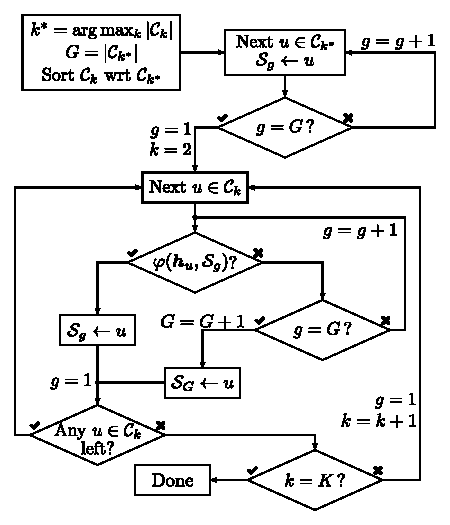
\includegraphics[width=.92\linewidth]{usch_figs/ClusterAssitedSchedulingAlgorithm.pdf}
	\caption{Flowchart of our proposed similarity-assisted greedy scheduling algorithm, using rule (\ref{eqn:assignment_rule_mac}) for downlink and (\ref{eqn:assignment_rule_bc}) for uplink.}
	\label{fig:similarity_assisted_scheduling}
\end{figure}

% \begin{algorithm}[htb]
% 	\caption{Greedy Similarity-Assisted User Gropuing}
% 	\label{alg:greedy_scheduling}
% 	\begin{algorithmic}[1]
% 		\Statex {\textbf{Input: }$\bm{h}_n\in\mathbb{C}^M,\,n\in\{1,\ldots,N\}$, clusters $\mathcal{C}_k,\,k\in\{1,\ldots,K\}$, correlation threshold $\beta$ }
% 		\State{Select largest cluster $\mathcal{C}_k^*$ and set $G=|\mathcal{C}_k^*|$}
% 		\State{Assign all users in $\mathcal{C}_k^*$ to different groups $\{\mathcal{S}_g\}_{g=1}^G$}
% 		\State{Sort clusters by decreasing intercluster distance with $\mathcal{C}_k^*$}
% % 		\For{$k=2\ldots K$}
% 		\For{each cluster $\mathcal{C}_{j}$ in sorted order, ${k}\geq2$}
% 		    \For{each user $n \in \mathcal{C}_{k}$}
%     		    \For{$g=1\ldots G$}
%             		\If {$\varphi(\bm{h}_n,\mathcal{S}{g})=1$}
%                         \State User $n$ is assigned to group $\mathcal{S}$
%                         \State \textbf{break}
%                     \EndIf
%                     \If {user has not been assigned yet}
%                         \State $G=G+1$
%                         \State Assign user $n$ to new group $\mathcal{S}_G$
%                     \EndIf
%         		\EndFor
% 		    \EndFor
% 		\EndFor
% 	\end{algorithmic}
% \end{algorithm}


For the sake of comparison, we implement a direct greedy scheduling approach that follows the same procedure, but has no clustering information, shown in Fig.\ref{fig:direct_greedy_scheduling}.
\begin{figure}[tbp]
	\centering
	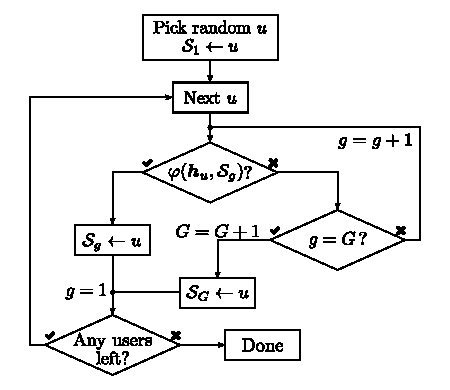
\includegraphics[width=.92\linewidth]{usch_figs/SchedulingAlgorithm.pdf}
	\caption{Flowchart of a direct greedy scheduling algorithm for benchmarking purposes following the same principles as our proposed algorithm.}
	\label{fig:direct_greedy_scheduling}
\end{figure}
% Algorithm~\ref{alg:direct_greedy_scheduling}.
% \begin{figure}
%     \centering
%     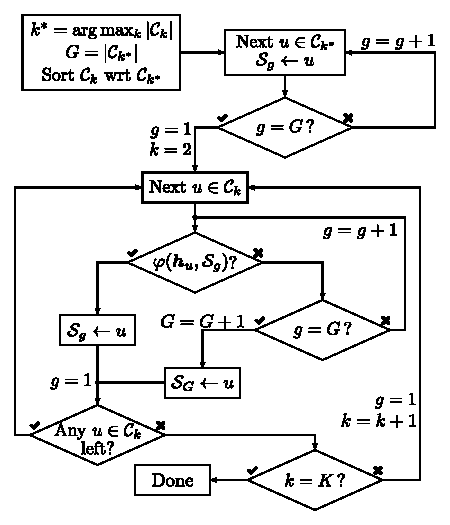
\includegraphics[width=\linewidth]{usch_figs/ClusterAssitedSchedulingAlgorithm.pdf}
%     \caption{Flowchart of our proposed similarity-assisted scheduling algorithm, using rule (\ref{eqn:assignment_rule_mac}) for downlink and (\ref{eqn:assignment_rule_bc}) for uplink.}
%     \label{fig:similarity_assisted_scheduling}
% \end{figure}
% \begin{algorithm}[htb]
% 	\caption{Greedy Direct User Gropuing}
% 	\label{alg:direct_greedy_scheduling}
% 	\begin{algorithmic}[1]
% 		\Statex {\textbf{Input: }$\bm{h}_n\in\mathbb{C}^M,\,n\in\{1,\ldots,N\}$, correlation threshold $\beta$ }
% 		\State{$G=1$ and pick a random user and assign to group $\mathcal{S}_1$}
% 	    \For{each remaining user $n$}
% 		    \For{$g=1\ldots G$}
%         		\If {$\varphi(\bm{h}_n,\mathcal{S}{g})=1$}
%                     \State User $n$ is assigned to group $\mathcal{S}_g$
%                     \State \textbf{break}
%                 \EndIf
%                 \If {user has not been assigned yet}
%                     \State $G=G+1$
%                     \State Assign user $n$ to new group $\mathcal{S}_G$
%                 \EndIf
%     		\EndFor
% 	    \EndFor
% 	\end{algorithmic}
% \end{algorithm}

Note that in both algorithms, the group rejection/assignment criterion can change from pairwise correlation to any other rule, such as setting a threshold for the SINR the user $n$ experiences when added to group $g$, which can be understood as outage management.



% \subsection{\textcolor{blue}{Channel Cluster Re-balancing}}
% More intuitively, based on the initial clustering results obtained from unsupervised learning, we can split big clusters by considering that there are maximum time slots per cluster and merge small clusters to achieve a nearly balanced cluster size.\ 

% Specifically, we use inter-cluster distance and intra-cluster distance as  metrics to identify the stability and effectiveness of the clustering result. In Phase 1, for big size clusters, for example $\mathcal{C}_k$, if the number of members is larger than the available time slots $N_{\rm{slot}}$, we will first split the $|\mathcal{C}_k|-N_{\rm{slot}}$ users with the largest intra-cluster distance as a new cluster. Then, given its neighboring cluster $\mathcal{C}_j$, their inter-cluster distance is $\varphi(\mathcal{C}_k, \mathcal{C}_j)$ and intra-cluster distance are $\psi(\mathcal{C}_k)$ and $\psi(\mathcal{C}_j)$. Following our scheduling strategy, users in the two neighboring cluster have high possibilities to be assigned into one user group. However, if it happens that $\psi(\mathcal{C}_k)>\varphi(\mathcal{C}_k, \mathcal{C}_j)$, there would exist some users in $k$-th cluster have larger distance to its partners in the same cluster than the users in cluster $\mathcal{C}_j$. Hence, we will identify these users and split them from the $k$-th cluster to avoid MAI resulted from possible user grouping. After that, in Phase 2,  for small size clusters or their subsets under the maximum allowable cluster size, if the average of their intra-cluster distance is larger than their inter-cluster distance, we will merge them into one cluster. The detailed flowchart for the dynamic adjustment in cluster splitting/merging is presented in Fig. \ref{dynamic_cluster}. 




% \subsection{\textcolor{blue}{Inter-cluster Distance Based User Grouping}}\label{icdug}
% As a matter of fact, the group capacity not only depends on the spatial correlation among the channels but also on the channel conditions of users. It is desirable to assign users with similar channel conditions into one group to counter near-far problem.

% The well known near-far effect is a special case of MAI when
% MAC users have significant difference in terms of the
% product between signal power and CSI gain, i.e.,
% $\sqrt{p_m}\|\bm{h_m}\|$. 
% In a near-far scenario, users with large power and CSI gain
% products tend to generate very strong MAI on users with
% small products.  Although power control to elevate
% the weaker user power can potentially
% alleviate the near-far effect, it comes at the cost
% of low power efficiency and worsening
% inter-cell interference. For this reason, in our design
% of MAC user scheduling groups, we would also
% form user groups by selecting users from different
% CSI clusters with similar CSI gain.\

% Instead of randomly selecting users from each cluster $\mathcal{C}_k, k \in\{1, \cdots, K\}$, \textcolor{blue}{after channel cluster rebalancing,} we exploit the channel gain information within each cluster, and the inter-cluster distance (ICD) between clusters. In Fig. \ref{scheme}, starting from the cluster with the largest number of users, we determine the neighboring cluster with the maximal ICD. Then, we select the user with the highest channel gains from each cluster and compose them as a spectrum sharing group. By repeating this step, we finally obtain the optimized user scheduling matrix $\bf{\Pi}$ as well as the user groups set $\mathcal{G}$ under the maximum access user limit $N$.\ 

% After that, to further improve the spectral efficiency, we merge small groups into a large group under the limitation of available time slots, therefore the users originally scheduled in a time slot with low utilization, i.e., the unsaturated user groups, would be assigned to other time slots. Here, one important issue is how to define the strategy or criteria for group merging. Specifically, given a fixed number of time slots $N_{\rm{slot}}$, the number of preferable user groups is known. Specifically, when the number of user groups $|\mathcal{G}|$ is larger than $N_{\rm{slot}}$, we will find the group set $\mathcal{G}'$ where the number of each group is less than $N$. Then, for any two groups from $\mathcal{G}'$, denoted by $\mathcal{G}_i$ and $\mathcal{G}_j$, we merge them if the total user number satisfies the maximum number constraint; Otherwise, we will choose the best subset, which has the largest capacity gain, from the $\mathcal{G}_j$, and merge it into $\mathcal{G}_i$. The above process repeats until the number of user groups is equal to the number of time slots. The detailed flowchart for the dynamic adjustment in group merging is presented in Fig. \ref{flow-regrouping}.


\subsection{Complexity Analysis}
\subsubsection{Clustering}
First, we determine the complexity of Grassmannian $K$-means as follows:
\begin{itemize}
	\item The CSI normalization step has a cost of $\mathcal{O}(MN)$.
	\item The Grassmannian distance has a cost of $\mathcal{O}(M)$, and thus the $k$-means++ initialization has a cost of $\mathcal{O}(KMN)$.
	\item Each iteration of the algorithm consists on two steps. First, assigning $N$ users to $K$ clusters, with a total cost of $\mathcal{O}(KMN)$. Then, the cluster center update for $K$ clusters, which requires the computation of $N$ logarithm maps and $K$ exponential maps, both operations with a cost of $\mathcal{O}(M)$. This process is iterative, but in practice takes only a few intrinsic mean iterations and the cost of center updates is $\mathcal{O}(KMN)$.
\end{itemize}
Accordingly, the total cost for $t$ iterations
of  Grassmannian $K$-means is $\mathcal{O}(tKMN)$.

In the case of Agglomerative Hierarchical Clustering, optimal implementations depend on the linkage criteria \cite{zaki14}.
When considering complete linkage, it is known that the optimal algorithm has complexity $\mathcal{O}(N^2)$ with respect to similarity comparisons. Furthermore, the pairwise CSI correlation has a total cost of $\mathcal{O}(MN^2)$ as there are $N(N-1)$ pairwise computations, and thus the complexity of this clustering approach is $\mathcal{O}(MN^2)$.

\subsubsection{User Grouping}
Both user grouping approaches (similarity-assisted and direct) exploit pairwise correlation information, which has cost $\mathcal{O}(M)$.
For the similarity-assisted approach, the algorithm checks $K-1$ clusters with a total of $N'=N-|\mathcal{C}_k^*|$ users, which we can approximate in average with an uniform partition as $N'=N-N/K=N(K-1)/K$. In the case of the direct pairwise-based greedy scheduling, there is no clustering information, and hence $N-1$ users need to be tested for assignment.
Hence, the computation complexity of both similarity-assisted and direct grouping is of order $\mathcal{O}(MN)$. Of course, in average we expect to observe some computational gains of similarity-assisted grouping, depending on system parameters and selected threshold, but cannot guarantee that they are going to be dramatically significant.

\section{Numerical Experiments}\label{sec:USCH_sim}
In this section we aim to show how the clustering step aids in scheduling. However, there is a large number of parameters that could impact the performance, such as different rate requirements of users or user channel gain. Therefore, we work on a simple system model.

% Fig. \ref{com6} shows the spectrum efficiency comparisons of PD based strategies with or without optimizing the value of $K$. In the cases without optimizing $K$, we set $K=N$. While in the cases with optimizing $K$, labeled by $K^\star$, we search $K$ from 2 to $N$, and choose the best one with the largest Silhouette coefficient. From Fig. \ref{com6}, we can observe that the performance gap between the dark solid lines and the blue dotted lines are small, especially when the number of users is small or the number of antennas is large. Nevertheless, since we need to compare the clustering results of each possible $K$, such optimization results in a high computation complexity. In the following, we apply the clustering algorithms without the determination of $K$ and set $K=N$.

We consider one BS equipped with $M$ antennas and $N$ users. The user CSIs are modeled as random channel vectors that consider both shadow and Rayleigh fading. A circularly complex normal vector of size $M$ represents MIMO Rayleigh fading, and shadow fading is represented as a power variable that follows a lognormal distribution in natural scale, with zero mean and standard deviation $\sigma_L$ of 3dB in logarithmic scale. Finally, the channels are normalized to have unit power to define an average SNR. Overall, the channel model is given by
\begin{align}
	\bm{h}_n=\frac{a_n}{\sqrt{\mathbb{E}\{\|\bm{v}_n\|^2\}\mathbb{E}\{a_n^2\}}}\bm{v}_n,\,\, &\bm{v}_n\sim\mathcal{CN}(\bm{0},\bm{I}_M),
%	\nonumber\\&
	\,\,
	a_n^2\sim\mathrm{Lognormal}(0,\sigma_L^2),
	% a_n\sim\mathrm{Lognormal}\Big(0,\big(\sigma_L\ln(10)/20\big)^2\Big)
	% \mathbb{E}\{\|\bm{v}\|\} = \frac{\Gamma\big(M+1/2\big)}{\Gamma(M)}
	\label{eqn:channel_model}   
\end{align}
and we set $\sigma^2=0.01$, which corresponds to 20dB of average SNR (i.e., whenever the channel gain is equal to 1). To ensure that results are independent of the chosen noise floor, we set the correlation threshold $\beta$ as a function of $\sigma$. 
% Unless explicitly stated, we set $M=8$ and $N=400$.


\subsection{Clustering Performance}

We notice that our chosen clustering algorithms require the pre-determination of the number $K$ of clusters. However, choosing $K$ is a difficult problem in clustering analysis, and there is no agreed-upon solution \cite{gap}. There are several methods to determine the optimal number of clusters, such as the Silhouette value \cite{silhouette}, the Krzanowski-Lai index \cite{Lai}, and the Hartigan index \cite{Hartigan}. Regardless, we know that the nature of the MAC and MU-MIMO systems imply that resource-sharing groups cannot have more than $M$ users, as having more users yields a rank-deficient group CSI matrix, impacting performance significantly. Hence, and knowing that there are much more users than BS antennas, we set $K=M$. As shown in Fig.~\ref{fig:clusters_pwc_M8_N400}, even with a suboptimal choice of $K$, clustering still provides useful similarity information to be used later in the scheduling process.

\begin{figure}[tb]
	\centering
	\begin{subfigure}[b]{0.49\linewidth}
		% Caption before figure
		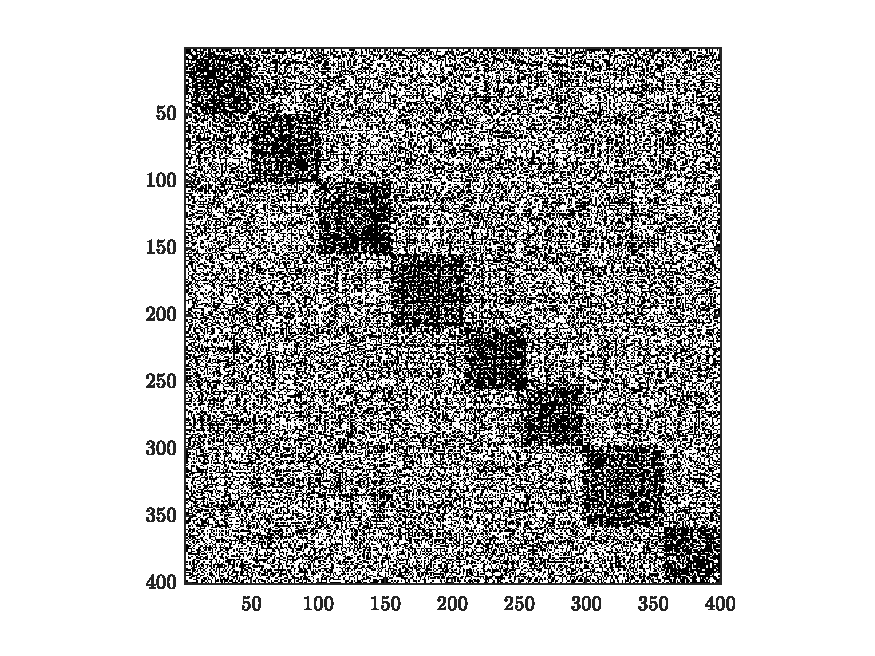
\includegraphics[width=\linewidth]{./usch_figs/pairwise_corr_all_users_GKM_threshold_M8_N400_K8.pdf}
		\subcaption{GKM.}\label{fig:pwc_gkm}
	\end{subfigure}\hfill
	\begin{subfigure}[b]{0.49\linewidth}
		% Caption before figure
		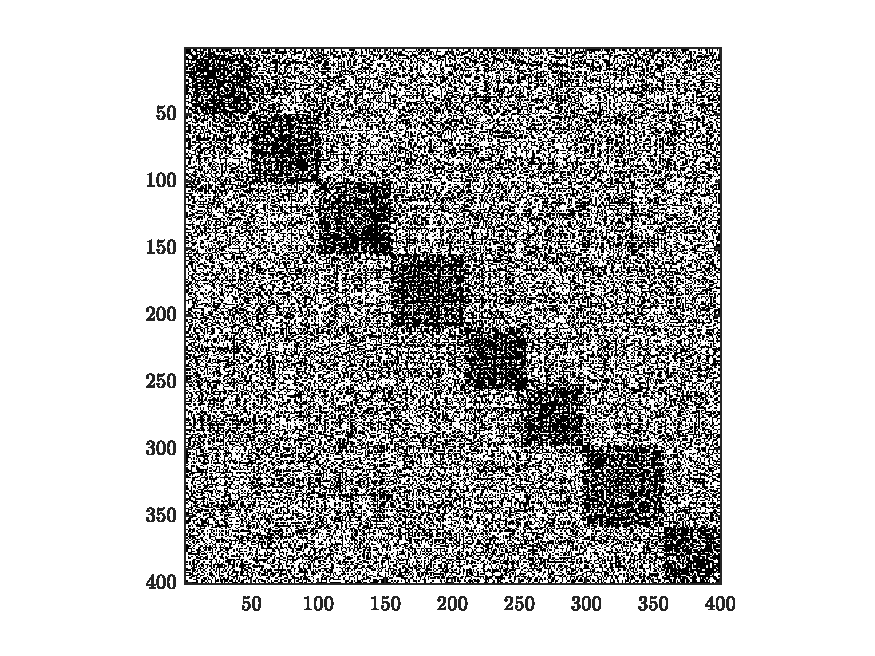
\includegraphics[width=\linewidth]{./usch_figs/pairwise_corr_all_users_AHP_threshold_M8_N400_K8.pdf}
		\subcaption{AHP.} \label{fig:pwc_AHP}
	\end{subfigure}\hfill
	\caption{Example of pairwise correlation matrices after clustering with $M=K=8$, $N=400$, and threshold $\beta=0.3\sigma$. Black values are larger than the threshold, white are lower. 
		(\subref{fig:pwc_gkm}) Grassmannian $K$-means. (\subref{fig:pwc_AHP}) Hierarchical Clustering. Even with non-optimum $K$, both approaches form clusters of users that share high similarity.}
	\label{fig:clusters_pwc_M8_N400}
\end{figure}


\begin{table}[h]
	\centering    
	\caption{Computational effort of clustering algorithms.}
	\label{tab:clustering_complexity_v}
	\begin{tabular}{c|c|cc|cc}
		$N$ & Measure & \multicolumn{2}{c|}{GKM} & \multicolumn{2}{c}{AHP} \\\hline
		\multirow{2}{*}{400}
		& Distances & 245131.2 & (\%)  & 79800 &(0\%)  \\ \cline{2-6}
		& Intrinsic Mean & 1228.37 &(\%)  & 136.184 &(\%)  \\ \hline
		\multirow{2}{*}{2000}
		& Distances &   & ( \%)  &  & (\%)  \\ \cline{2-6}
		& Intrinsic Mean &  & ( \%) &  &(\%)  \\ \hline
	\end{tabular}
\end{table}


\subsection{Scheduling Performance Metrics}
\subsubsection{Interference}
We compute the loss in SINR that each user experiences. In other words, the normalize the SNIR of user $n$ by the SNR of user $n$ if it were scheduled with no other users (a singleton group), such that it does not share resources and whose signal is only distorted by noise, that is,
\begin{align}
	\frac{\SINR_n}{p_n\|\bm{h}_n\|^2/\sigma^2}.\label{eqn:normalized_sinr}
\end{align}
Thus, 0dB of loss corresponds to the SNR experienced by an user in a singleton group, i.e. that is not sharing resources.
% \textcolor{red}{PLEASE Show numerical results in figures}
\subsubsection{Total sum rate}
In each channel realization and simulation, we compute the total sum capacity by summing the capacity of all groups. 
In BC scenarios, we add the rate of all users, each normalized by the rate that the user would achieve with no interference, i.e.,
\begin{align}
	R^{\BC}=\sum_{g=1}^G\sum_{n\in\mathcal{S}_g}\frac{\log_2(1+\SINR_n^{\BC})}{\log_2(1+p_n\|\bm{h}_n\|^2/\sigma^2)}.\label{eqn:normalized_sumcap_bc}
\end{align}

In MAC, the grouping rule considers the grouping of users with similar channel gains to guarantee a proper MMSE receiver performance. Thus, here we normalize the capacity of each group $g$ by the rate achieved by a virtual reference user with channel gain equal to the average channel gain $\hat{b}_g$ in partition $b(\mathcal{S}_g)$. Thanks to the channel gain partitioning, the transmission power can be controlled at the group level and set a power level $\hat{p}_g$ for all users in grup $g$ to further control the sum capacity. Therefore, the normalized sum capacity in MAC is given by
\begin{align}
	R^{\MAC}=\sum_{g=1}^G\frac{C_g^{\MAC}}{\log_2(1+\hat{p}_g\hat{b}_g^2/\sigma^2)}.\label{eqn:normalized_sumcap_mac}
\end{align}

\subsubsection{Resource Efficiency}
To measure how each scheme is using resources to serve users, we divide the total sum capacity over the number of groups used by each algorithm in each case, i.e.,
\begin{align}
	\frac{1}{G}\sum_{g=1}^G C_{g}.
\end{align}
% We will also evaluate the worst individual rate of users, which is a more realistic measure than the average performance in some applications.

\subsubsection{Computational scheduling effort}
As a proxy for computational complexity, in all simulations we store the amount of tries to assign all users to groups in the scheduling process. This allows to empirically corroborate which approach requires less computation steps, and if the clustering step does really provide an advantage.




% We consider different scenarios, as described in Table~\ref{table:scenarios}.





\subsection{Performance for Uplink (MAC)}
In MAC, we analyze our approach with and without power control, as power control is more critical for the sake of proper performance of the MMSE receiver and user fairness. We define two scenarios:
\begin{enumerate}
	\item one where all CSI have unit power, i.e. $\|h_n\|^2=1\,\forall n\in\{1,\ldots,N\}$, which we call MAC-U; and
	\item another where all CSI have gains given by the random realizations of the channel according to Eq.(\ref{eqn:channel_model}), which we denote MAC-P.
\end{enumerate}



% Comments:
% threshold = 1 -> no correlation whatsoever, greedy is essentially random. GKM and AHP does no rejection, but is based in clustering only (clustering helps, and
% Threshold = 0 

First we analyze the MAC-U scenario, which is of interest as it helps to isolate the contributions of our strategy without the effect of variable channel powers. 
Fig.~\ref{fig:MACU_sinrLoss_M8_N400} shows the average SINR loss of users is equivalent for all scheduling approaches when the correlation threshold $\beta$ is small, which is the dominant scheduling rule in this regime. In other words, the process is driven by the correlation threshold portion of the scheduling rule (\ref{eqn:assignment_rule_mac}). However, when $\beta$ increases, the SINR loss is controlled in the similarity-assisted schemes GKM and AHP, whereas the direct approach yields increasingly worse conditions for users, as they average losses of up to 8dB of SINR, compared to 2dB for GKM and 1dB for AHP. 


The average normalized sum capacity given by Eq.(\ref{eqn:normalized_sumcap_mac}) is shown in Fig.\ref{fig:MACU_sumcapacity_M8_N400}. In correspondence with the SNIR results from Fig.\ref{fig:MACU_sinrLoss_M8_N400}, the sum capacity of all approaches is very similar for low values of $\beta$, but drastically changes when $\beta$ increases. Both GKM and AHP are able to control the sum capacity decrease by exploiting similarity information with a loss of about 5-10\%, and the direct approach experiences up to a 40\% of capacity loss.


The achieved efficiency of MAC-U is shown in Fig.\ref{fig:MACU_efficiency_M8_N400}. This measure differs from the sum capacity as it depends on the number of resource-sharing groups needed in each scheme to service all users. For lower values of $\beta$, the efficiency of all scheduling approaches is essentially the same, reinforcing the idea that in this regime, the threshold value $\beta$ becomes the dominant criteria for scheduling. However, when $\beta$ increases, we can observe that AHP starts suffering first, as it usually requires more groups in the allocation process. The direct approach, even requiring the least amount of groups, now has a lower sum capacity and the efficiency decreases. GKM is able to leverage the similarity information, yielding better efficiency than the other approaches.
\begin{figure}[tb]
	\centering
	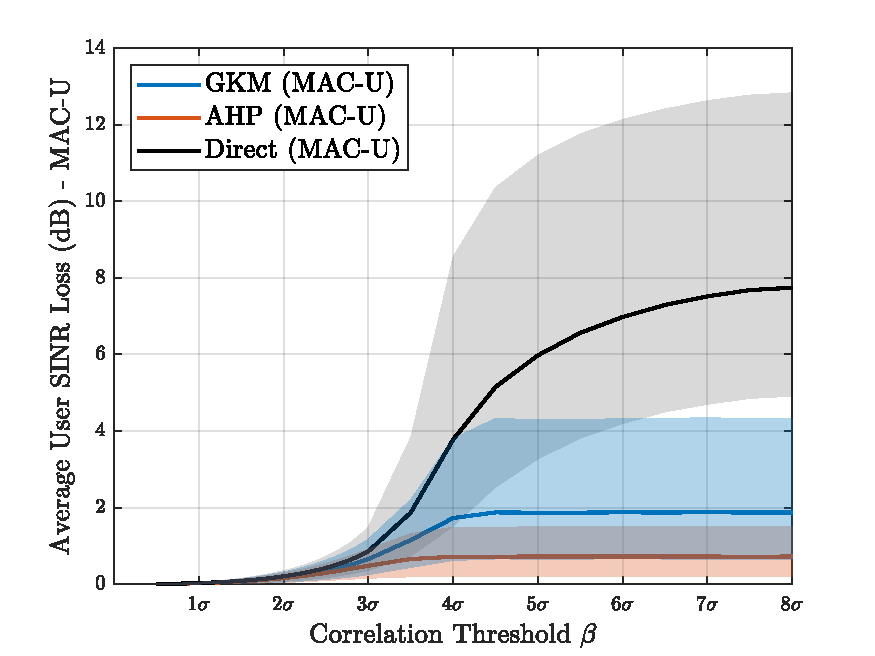
\includegraphics[width=.5\linewidth]{./usch_figs/MACU_AvgUserSINRLoss_normalizedChannelPwr_M8_N400_nSim50_nChannel100_K08_sigman2_1em1.pdf}
	\caption{Average normalized user SINR loss in unit-gain MAC for different scheduling approaches. The solid line represents the average over channel realizations, and the shaded area shows all values within the 10th and 90th percentiles. Larger loss means that the users experience worse conditions. Here, $M=K=8$ and $N=400$.}
	\label{fig:MACU_sinrLoss_M8_N400}
\end{figure}
\begin{figure}[tb]
	\centering
	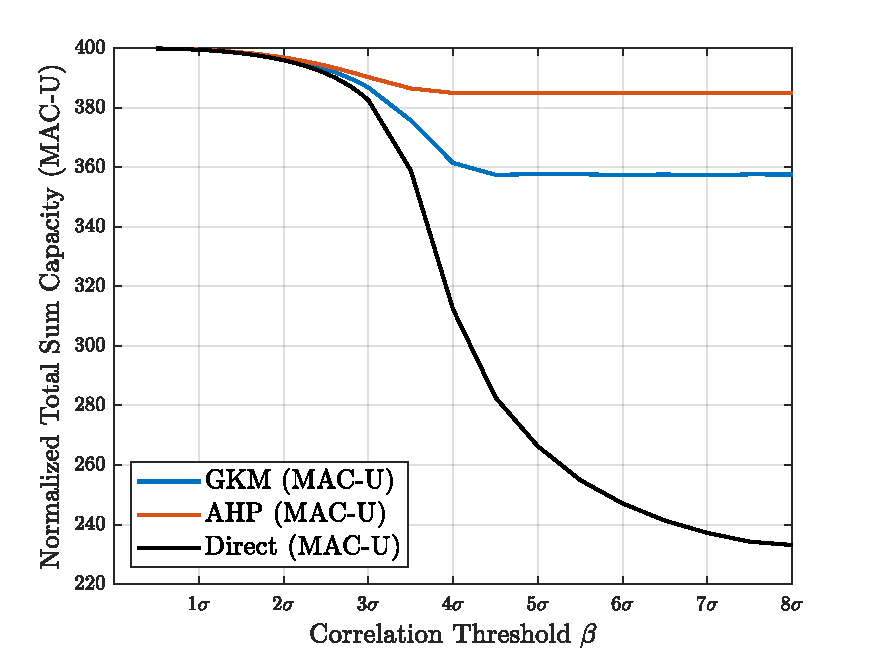
\includegraphics[width=.5\linewidth]{./usch_figs/MACU_NormalizedSumCap_normalizedChannelPwr_M8_N400_nSim50_nChannel100_K08_sigman2_1em1.pdf}
	\caption{Average normalized sum capacity in unit-gain MAC for different scheduling approaches. Here, $M=K=8$ and $N=400$.}
	\label{fig:MACU_sumcapacity_M8_N400}
\end{figure}
\begin{figure}[tb]
	\centering
	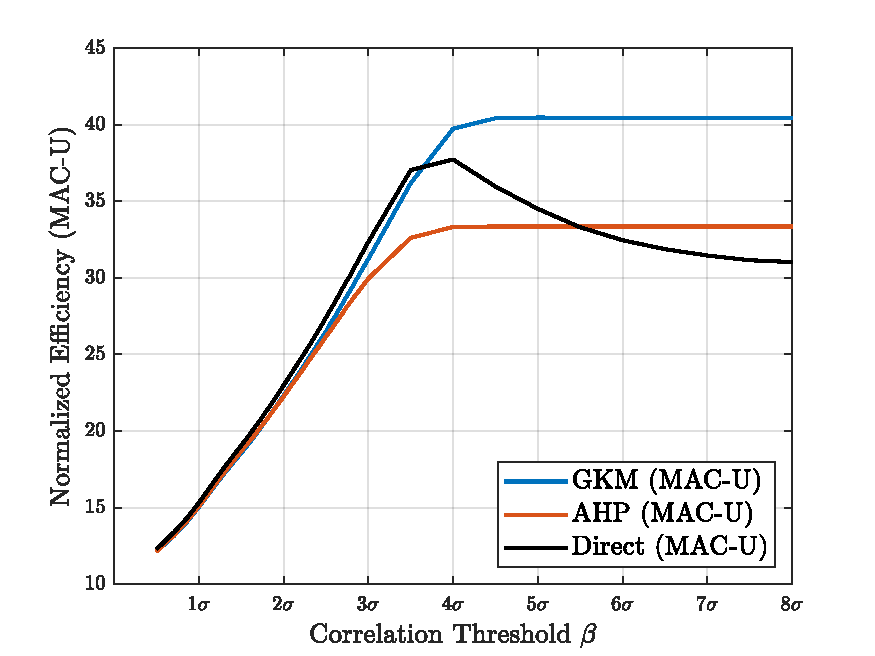
\includegraphics[width=.5\linewidth]{./usch_figs/MACU_NormalizedEfficiency_normalizedChannelPwr_M8_N400_nSim50_nChannel100_K08_sigman2_1em1.pdf}
	\caption{Average efficiency in unit-gain MAC for different scheduling approaches. Here, $M=K=8$ and $N=400$.}
	\label{fig:MACU_efficiency_M8_N400}
\end{figure}



\begin{figure}[tb]
	\centering
	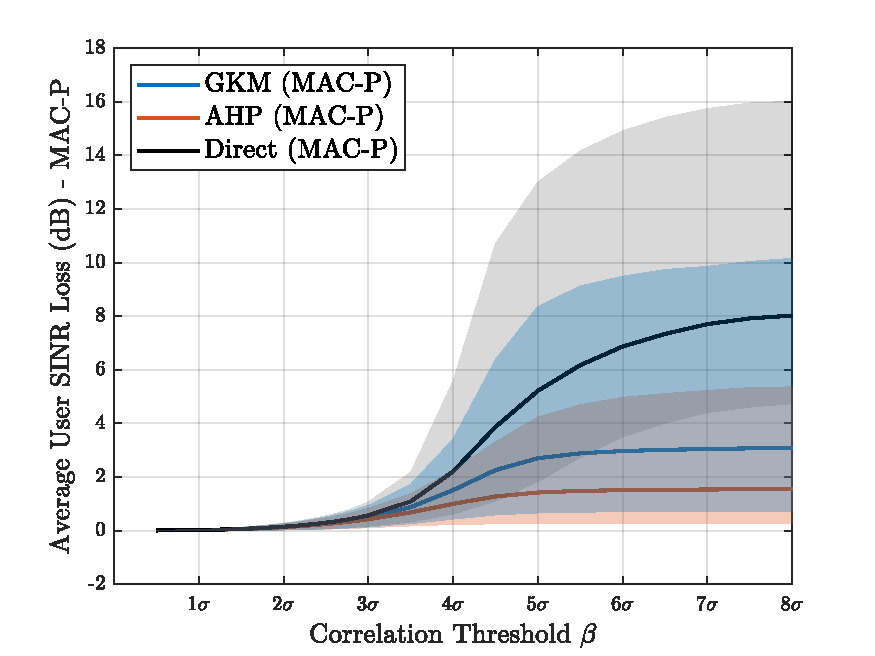
\includegraphics[width=.5\linewidth]{./usch_figs/MACP_AvgUserSINRLoss_normalizedChannelPwr_M8_N400_nSim50_nChannel100_K08_sigman2_1em1.pdf}
	\caption{Average normalized user SINR loss in gain-control MAC for different scheduling approaches. The solid line represents the average over channel realizations, and the shaded area shows all values within the 10th and 90th percentiles. Larger loss means that the users experience worse conditions. Here, $M=K=8$ and $N=400$.}
	\label{fig:MACP_sinrLoss_M8_N400}
\end{figure}
\begin{figure}[tb]
	\centering
	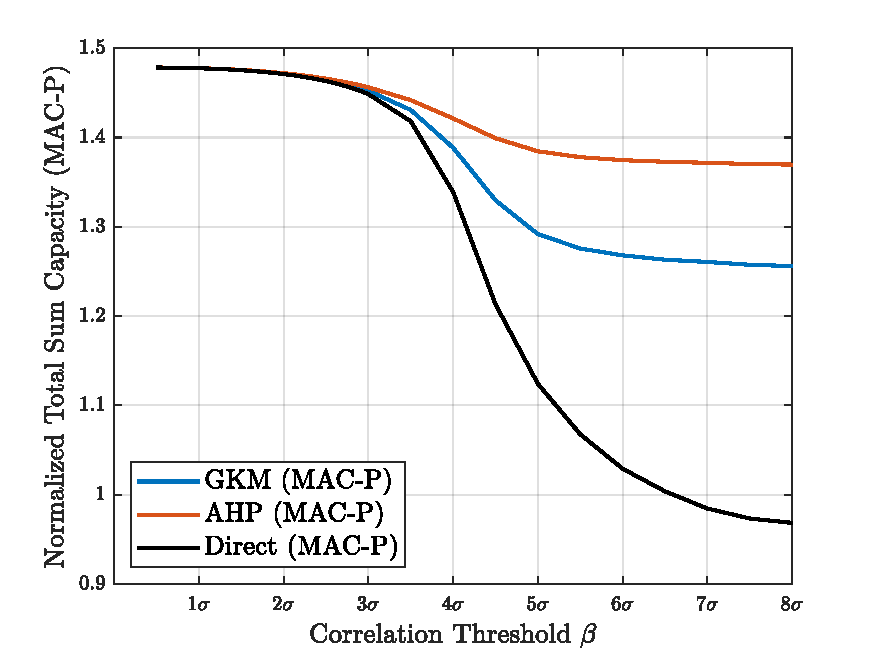
\includegraphics[width=.5\linewidth]{./usch_figs/MACP_NormalizedSumCap_normalizedChannelPwr_M8_N400_nSim50_nChannel100_K08_sigman2_1em1.pdf}
	\caption{Average normalized sum capacity in gain-control MAC for different scheduling approaches. Here, $M=K=8$ and $N=400$.}
	\label{fig:MACP_sumcapacity_M8_N400}
\end{figure}
\begin{figure}[tb]
	\centering
	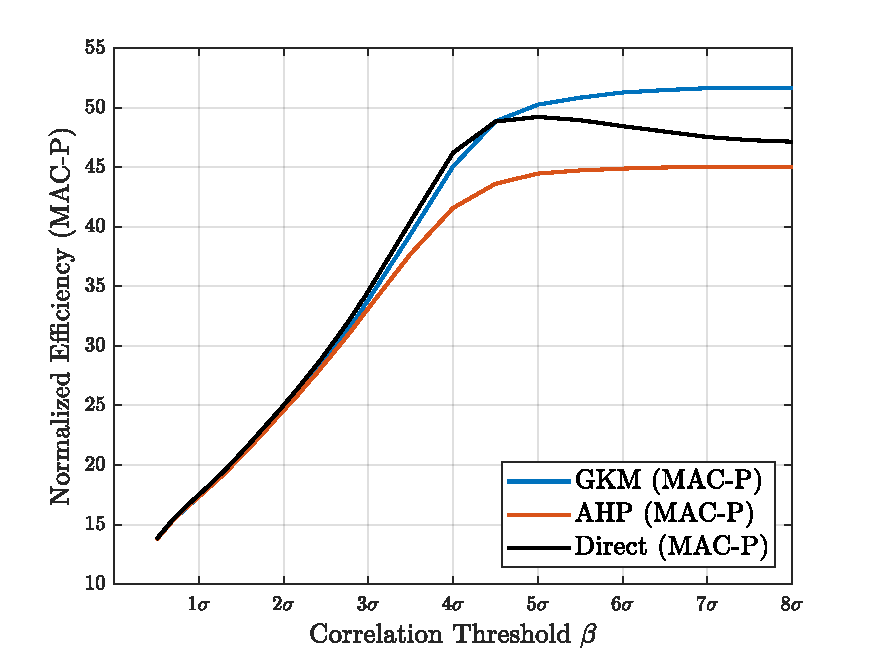
\includegraphics[width=.5\linewidth]{./usch_figs/MACP_NormalizedEfficiency_normalizedChannelPwr_M8_N400_nSim50_nChannel100_K08_sigman2_1em1.pdf}
	\caption{Average efficiency in gain-control MAC for different scheduling approaches. Here, $M=K=8$ and $N=400$.}
	\label{fig:MACP_efficiency_M8_N400}
\end{figure}
Fig.\ref{fig:MACP_sinrLoss_M8_N400} shows the SINR loss in the case with variable CSI gains (MAC-P). When including channel gains, the similarity-assisted schemes experience in average 1dB more of loss compared to the MAC-U case, whereas the direct approach behaves similarly in average. Nevertheless, there is still a gap of 5dB when comparing GKM with the direct approach. Additionally, the distribution of SINR loss spreads for all schemes, resulting in more users with worse SINR conditions. However, the direct approach yields the worst results, whereas in comparison GKM and AHP are able to improve the quality of service of users with worse conditions with an increase of up to 6dB in SINR. 

In Fig.\ref{fig:MACP_sumcapacity_M8_N400} we present the average normalized sum capacity for MAC-P. Again, our results confirm that the direct approach will suffer the most with increasing $\beta$, with capacity decreasing by a losses up to 50\% of its maximum value. On the other hand, GKM can control the capacity decreases only to 17\%, and AHP only an 8\%.


Finally, we present the he achieved efficiency of MAC-P in Fig.\ref{fig:MACP_efficiency_M8_N400}. Here, the results show a similar behavior as in MAC-U: With lower values of $\beta$, the efficiency of all scheduling approaches is essentially the same, with AHP being the worse due to allocating more groups in the process. For larger values of $\beta$, the direct approach again fails to keep up with GKM in terms of efficiency, with GKM having up to 9.5\% better performance. 


The number of assignment attempts needed in each scheme to schedule all users are summarized in Table~\ref{tab:assign_attempts_mac_v} with representative values of $\beta$.
All values for similarity-assisted scheduling are also shown as a percentage of the values of the direct approach for comparison.
Overall, AHP requires the least amount of attempts, followed closely by GKM. In unit-gain MAC, the reduction in attempts is quite significant, needing even less than 9\% of the direct scheduling attempts. In MAC-P, the reduction is not as sharp, but is still significant, shaving off at least 24\%. This means that the similarity information is indeed helping to avoid bad pairings that result in poor grouping.
% \begin{table}[]
%     \centering    
%     \caption{Average assign attempts to schedule all users in downlink experiments.}
%     \label{tab:assign_attempts_mac}
%     \begin{tabular}{l|c|c|c|c}
%          & \multicolumn{2}{c|}{MAC-U} & \multicolumn{2}{c}{MAC-P}\\\cline{2-5} 
%          & $\beta=4\sigma$ & $\beta=8\sigma$ & $\beta=4\sigma$ & $\beta=8\sigma$ \\ \hline
%          GKM & 439.1 (23.0\%)& 342.6 (8.2\%)& 3191.0 (75.5\%)& 2974.56 (58.8\%)\\
%          AHP & 327.5 (17.2\%)& 322.3 (7.5\%)& 2716.0 (64.2\%)& 2532.8 (50.0\%)\\
%          Direct & 1909.4 & 4271.3& 4227.7 & 5063.0\\
%     \end{tabular}
% \end{table}
% beta=1\sigma
% macu  
% gkm   14223.0 (92.3\%)
% ahp   12792.8 (83.0\%)
% direct 15411.5  
% macp  
% gkm  23043.6 (94.8\%)
% ahp  21726.0 (89.4\%)
% direct 24313.7 


\begin{table}[h]
	\centering    
	\caption{Average assign attempts to schedule all users in downlink experiments.}
	\label{tab:assign_attempts_mac_v}
	\begin{tabular}{c|c|cc|cc|c}
		Mode & $\beta$ & \multicolumn{2}{c|}{GKM} & \multicolumn{2}{c|}{AHP} & Direct \\\hline
		\multirow{3}{*}{MAC-U}
		& $1\sigma$ & 14223.0 &(92.3\%)  & 12792.8 &(83.0\%) & 15411.5   \\ \cline{2-7}
		& $4\sigma$ & 439.1 &(23.0\%) & 327.5 &(17.2\%)& 1909.4  \\ \cline{2-7}
		& $8\sigma$ & 342.6 &(8.2\%)  & 322.3 &(7.5\%) & 4271.3 \\ \hline
		\multirow{3}{*}{MAC-P}
		& $1\sigma$ & 23043.6 &(94.8\%) & 21726.0 &(89.4\%) & 24313.7  \\ \cline{2-7}
		& $4\sigma$ & 3191.0 &(75.5\%)  & 2716.0 &(64.2\%) & 4227.7  \\ \cline{2-7}
		& $8\sigma$ & 2974.56 &(58.8\%) & 2532.8 &(50.0\%) & 5063.0 \\ \hline
	\end{tabular}
\end{table}

\begin{figure}[tbp]
	\centering
	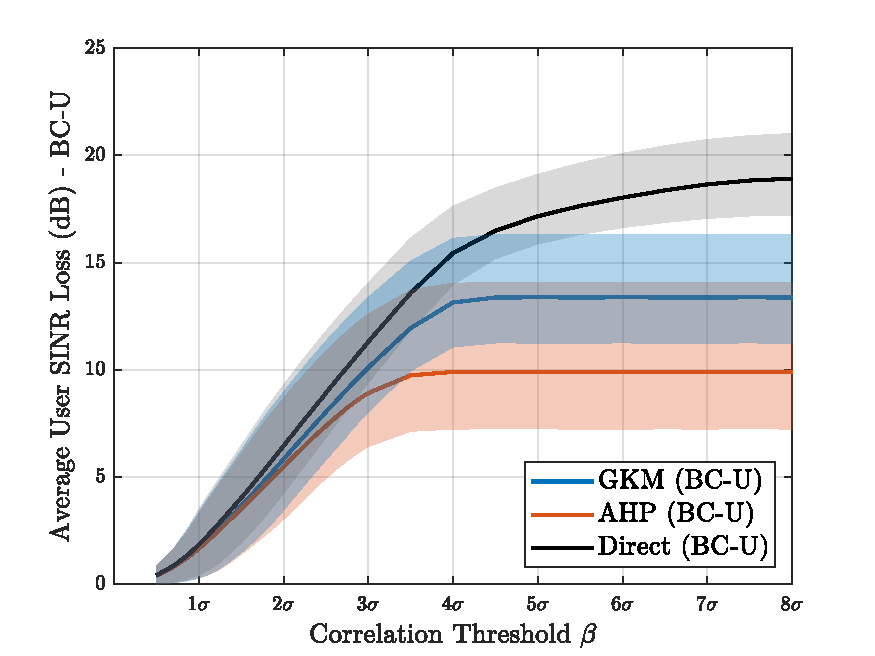
\includegraphics[width=.5\linewidth]{./usch_figs/BCU_AvgUserSINRLoss_normalizedChannelPwr_M8_N400_nSim50_nChannel100_K08_sigman2_1em1.pdf}
	\caption{Average normalized user SINR loss in unit-gain BC for different scheduling approaches. The solid line represents the average over channel realizations, and the shaded area shows all values within the 10th and 90th percentiles. Larger loss means that the users experience worse conditions. Here, $M=K=8$ and $N=400$.}
	\label{fig:BCU_sinrLoss_M8_N400}
\end{figure}
\begin{figure}[tbp]
	\centering
	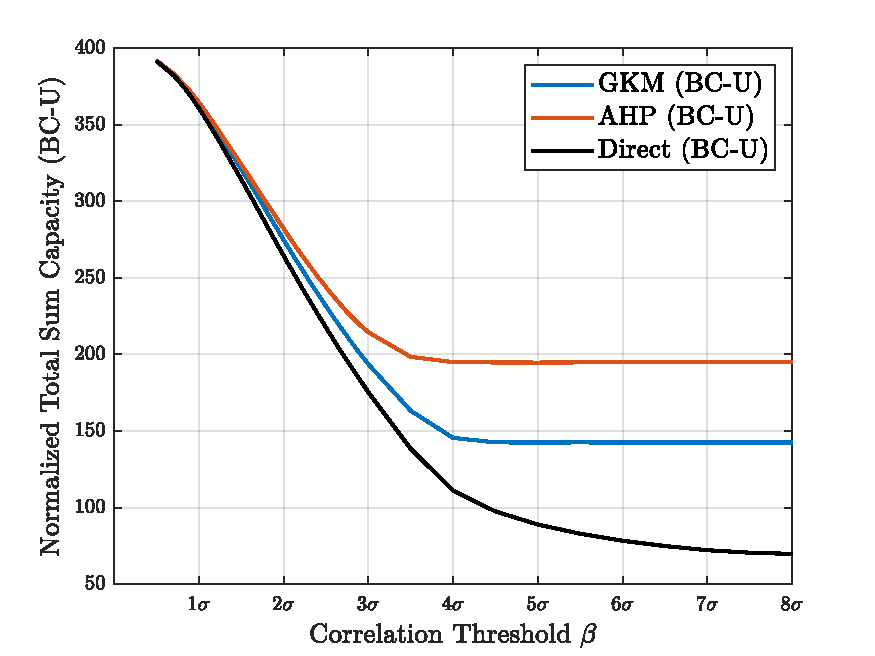
\includegraphics[width=.5\linewidth]{./usch_figs/BCU_NormalizedSumCap_normalizedChannelPwr_M8_N400_nSim50_nChannel100_K08_sigman2_1em1.pdf}
	\caption{Average normalized sum capacity in unit-gain BC for different scheduling approaches. Here, $M=K=8$ and $N=400$.}
	\label{fig:BCU_sumcapacity_M8_N400}
\end{figure}
\begin{figure}[tbp]
	\centering
	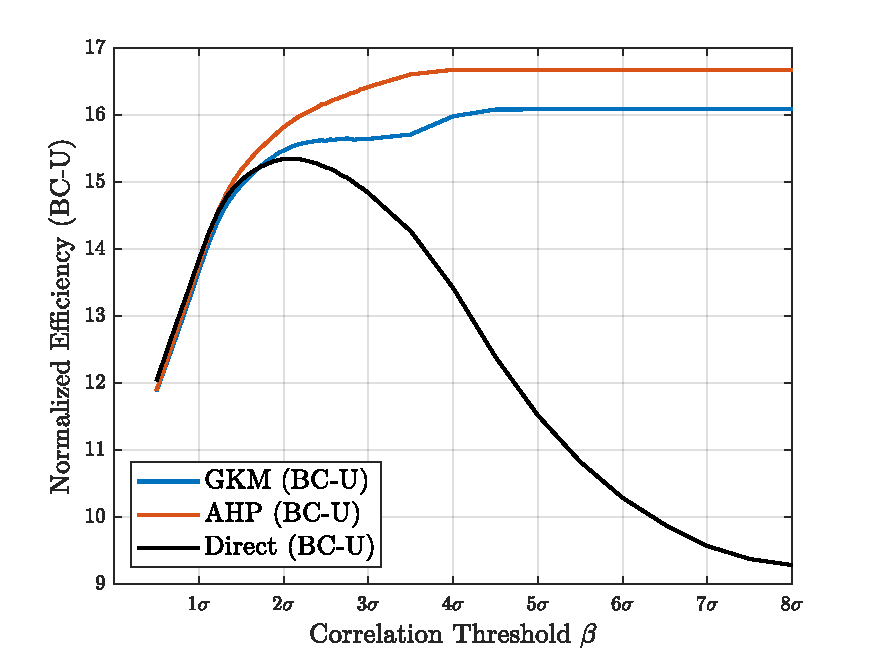
\includegraphics[width=.5\linewidth]{./usch_figs/BCU_NormalizedEfficiency_normalizedChannelPwr_M8_N400_nSim50_nChannel100_K08_sigman2_1em1.pdf}
	\caption{Average efficiency in unit-gain BC for different scheduling approaches. Here, $M=K=8$ and $N=400$.}
	\label{fig:BCU_efficiency_M8_N400}
\end{figure}
\subsection{Performance for Downlink (MU-MIMO)}
For the MU-MIMO scenario, we do not consider power control, and therefore all users have the same power $p_n=1$, $n\in\{1,\ldots,N\}$. For the purposes of analysis, we again consider two cases: 
\begin{enumerate}
	\item one where all CSI have unit power, i.e. $\|h_n\|^2=1\,\forall n\in\{1,\ldots,N\}$, which we call BC-U; and
	\item another where all CSI have gains given by the random realizations of the channel according to Eq.(\ref{eqn:channel_model}), which we denote BC-P.
\end{enumerate}



First we analyze the BC-U scenario. Again, the idea is to isolate the effect of channel gain in the analysis.
Fig.~\ref{fig:BCU_sinrLoss_M8_N400} shows the average SINR loss of users. Even with low values of $\beta$, the average SIN of each scheme can be distinguished, even when the SINR distribution is very similar for all approaches. The SINR values are worse than in MAC, which is expected as the users have no CSI information of other users and cannot mitigate interference with this knowledge (as it occurs with the MMSE receiver in MAC). Nevertheless, AHP is again yielding the best SINR conditions for users with losses averaging 10dB, and the direct approach the worst, with losses up to 19dB of SINR. GKM acts like a tradeoff, with losses up to 13dB.

The average normalized sum capacity given by Eq.(\ref{eqn:normalized_sumcap_bc}) is shown in Fig.\ref{fig:BCU_sumcapacity_M8_N400}. The achieved sum capacity is rather similar for low $\beta$, and decreases sharply with increasing threshold. AHP has its capacity decreased by up to 50\%, GKM decreases by up to 65\%, and the direct scheduling decreases sharply until reaching  up to 82\% of capacity decrease.

Fig.\ref{fig:BCU_efficiency_M8_N400} shows the attained efficiency of BC-U. As expected, the efficiency of all approaches is very similar for low values of $\beta$. With increasing $\beta$, the direct approach starts suffering due to the diminished sum capacity, decreasing sharply by a large margin until reaching 60\% of the maximum capacity that is able to achieve. Similarity-assisted schemes, on the other hand, are able to further increase the efficiency with larger $\beta$. with AHP showing the best result and GKM having only a small difference.


For BC-P, where channels have variable gains, Fig.\ref{fig:MACP_sinrLoss_M8_N400} shows the achieved SINR loss. When including channel gains, the distribution spread of all schemes increases, although average losses tend to be reduced in 2 to 3dB compared to BC-U. The gap between GKM and AHP decreases relative to BC-U, and the relative average gap between GKM and the direct approach \emph{increases}, and also becomes significant at lower values of $\beta$ compared to BC-U. The direct approach is again yielding the worst SINR conditions for users for almost all values of $\beta$. 

The average normalized sum capacity for BC-P is depicted in Fig.\ref{fig:BCP_sumcapacity_M8_N400}. The achieved sum capacity is rather similar for low $\beta$, and decreases sharply with increasing threshold. For low values of $\beta$, the direct scheme achieves slightly higher sum capacity, to then sharply decrease with increasing $\beta$. AHP and GKM perform similarly, with AHP yielding higher sum capacity across $\beta$ values. For AHP, the sum capacity decreases to 49.8\% of the maximum value, GKM decreases to 41.73\%, and the direct scheduling decreases sharply until reaching only 18.8\% of its maximum value.

Fig.\ref{fig:MACP_efficiency_M8_N400} shows the achieved efficiency of BC-P. Here, the efficiency of the direct approach is the highest for low values of $\beta$, while not significantly different from the similarity-based approaches. However, with increasing $\beta$, it peaks and then decreases to about the 60\% of its maximum value. On the contrary, both AHP and GKM enjoy increasing efficiency with increasing values of $\beta$, both surpassing the peak of the direct scheme, and only having a small gap between the two.

\begin{figure}[tbp]
	\centering
	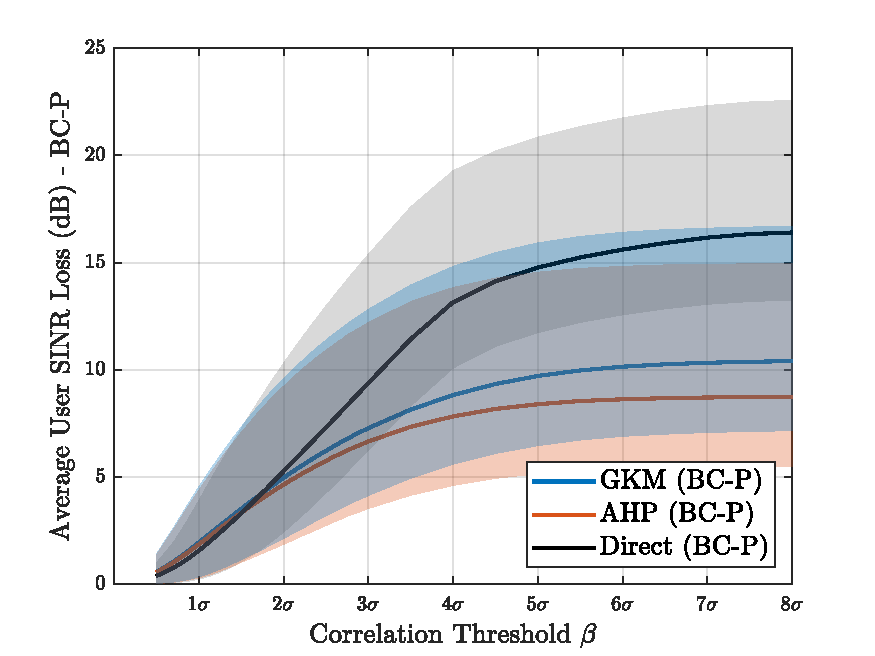
\includegraphics[width=.5\linewidth]{./usch_figs/BCP_AvgUserSINRLoss_normalizedChannelPwr_M8_N400_nSim50_nChannel100_K08_sigman2_1em1.pdf}
	\caption{Average normalized user SINR loss in random-gain BC for different scheduling approaches. The solid line represents the average over channel realizations, and the shaded area shows all values within the 10th and 90th percentiles. Larger loss means that the users experience worse conditions. Here, $M=K=8$ and $N=400$.}
	\label{fig:BCP_sinrLoss_M8_N400}
\end{figure}

\begin{figure}[tbp]
	\centering
	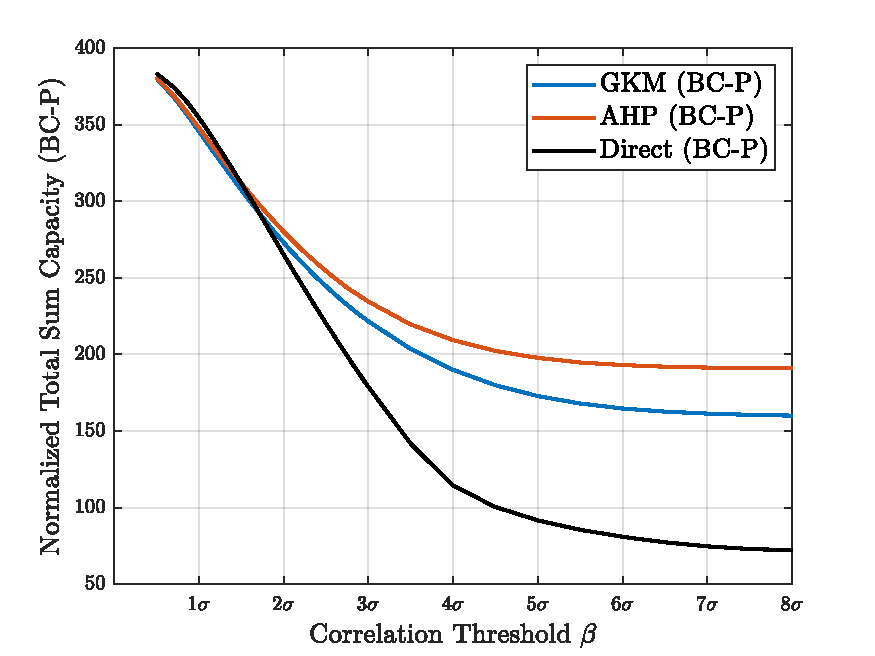
\includegraphics[width=.5\linewidth]{./usch_figs/BCP_NormalizedSumCap_normalizedChannelPwr_M8_N400_nSim50_nChannel100_K08_sigman2_1em1.pdf}
	\caption{Average normalized sum capacity in random-gain BC for different scheduling approaches. Here, $M=K=8$ and $N=400$.}
	\label{fig:BCP_sumcapacity_M8_N400}
\end{figure}


\begin{figure}[tbp]
	\centering
	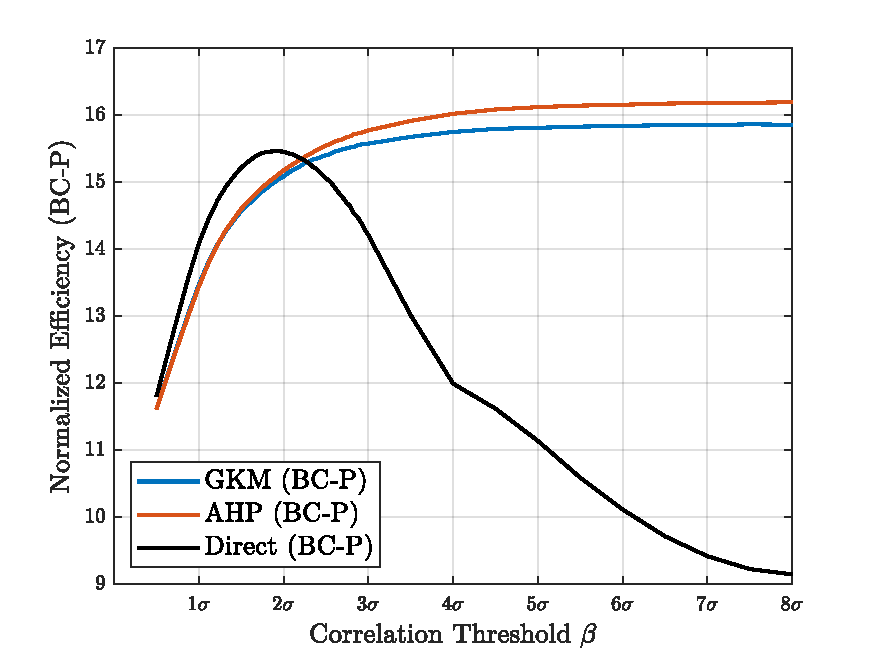
\includegraphics[width=.5\linewidth]{./usch_figs/BCP_NormalizedEfficiency_normalizedChannelPwr_M8_N400_nSim50_nChannel100_K08_sigman2_1em1.pdf}
	\caption{Average efficiency in random-gain BC  for different scheduling approaches, normalized by the total achievable capacity of a group with $M$ orthogonal users. Here, $M=K=8$ and $N=400$.}
	\label{fig:BCP_efficiency_M8_N400}
\end{figure}

We also show in Table~\ref{tab:assign_attempts_bc_v} the number of assignment attempts needed in each scheme to schedule all users.
Again, similarity information helps in scheduling, as AHP and GKM require less attempts that the direct approach. For BC-U, selecting a threshold of $4\sigma$ helps reducing the attempts in at least 77\%, and is able to keep reducing attempts to less than 8\% of the direct approach attempts. We see a similar behavior in BC-P, where the reduction is larger than in downlink MAC-P: 45\% or less of the attempts of direct scheduling are needed for increasing values of $\beta$. The similarity-assisted scheduling is further reducing computational complexity, and can easily compensate the added complexity of the clustering step.
% \begin{table}[]
%     \centering    
%     \caption{Average assign attempts to schedule all users in uplink experiments.}
%     \label{tab:assign_attempts_bc}
%     \begin{tabular}{l|c|c|c|c}
%          & \multicolumn{2}{c|}{BC-U} & \multicolumn{2}{c}{BC-P}\\\cline{2-5} 
%          & $\beta=4\sigma$ & $\beta=8\sigma$ & $\beta=4\sigma$ & $\beta=8\sigma$ \\ \hline
%          GKM & 437.3 (22.9\%)& 342.6 (8.0\%)& 1237.6 (55.2\%)& 357.3 (9.8\%)\\
%          AHP & 327.6 (17.1\%)& 322.3 (7.5\%)& 968.9 (43.2\%)& 330.969 (9.1\%)\\
%          Direct & 1911.7 & 4274.8& 2240.8 & 3653.1\\
%     \end{tabular}
% \end{table}
% beta=1\sigma
% bcu  
% gkm   14233.2 (92.3\%)
% ahp   12795.8 (83.0\%)
% direct 15407.7  

% bcp  
% gkm  11561.2 (87.8\%)
% ahp  11011.7 (83.6\%)
% direct 13172.4 
\begin{table}[htb]
	\centering    
	\caption{Average assign attempts to schedule all users in uplink experiments.}
	\label{tab:assign_attempts_bc_v}
	\begin{tabular}{c|c|cc|cc|c}
		Mode & $\beta$ & \multicolumn{2}{c|}{GKM} & \multicolumn{2}{c|}{AHP} & Direct \\\hline
		\multirow{3}{*}{BC-U}
		& $1\sigma$ & 14233.2 & (92.3\%) & 12795.8 & (83.0\%) & 15407.7 \\ \cline{2-7}
		& $4\sigma$ & 437.3 & (22.9\%) & 327.6 & (17.1\%) &  1911.7  \\ \cline{2-7}
		& $8\sigma$ & 342.6 & (8.0\%) & 322.3 & (7.5\%) &   4274.8   \\ \hline
		\multirow{3}{*}{BC-P}
		& $1\sigma$ & 11561.2 & (87.8\%) & 11011.7 & (83.6\%) & 13172.4   \\ \cline{2-7}
		& $4\sigma$ & 1237.6 & (55.2\%)  & 968.9 & (43.2\%) & 2240.8  \\ \cline{2-7}
		& $8\sigma$ & 357.3 & (9.8\%) & 330.969 & (9.1\%)  & 3653.1   \\ \hline
	\end{tabular}
\end{table}

